% @Author: Moez Bouhlel

\documentclass[
a4paper,
12pt,
%twoside,
onecolumn,
titlepage,
final,
]{report} % {scrartcl}

\usepackage[utf8]{inputenc}
\usepackage[T1]{fontenc}
\usepackage[shorthands=off,english,french]{babel}
%\usepackage[fixlanguage]{babelbib}
%\usepackage{polyglossia}
%\setmainlanguage{french}
%\setotherlanguages{english}
\usepackage{csquotes}
\usepackage{soul}

\usepackage{abstract}
\renewcommand{\abstractnamefont}{\large\bfseries}
\usepackage[toc,page]{appendix}
\renewcommand{\appendixtocname}{Annexes}

\usepackage[nottoc]{tocbibind}
\usepackage[style=alphabetic,backend=bibtex8]{biblatex}
\addbibresource{bibliography.bib}

\usepackage{ifxetex,ifluatex}

%\usepackage{mathspec}
\usepackage{amssymb,amsmath}

%\usepackage{xltxtra,xunicode}
%\defaultfontfeatures{Mapping=tex-text,Scale=MatchLowercase}
%\setmainfont{TeX Gyre Pagella}
%\setsansfont{FreeSans}
%\setmonofont[Mapping=tex-ansi]{Monaco}

\usepackage{color}
\usepackage[table]{xcolor}

\usepackage{lmodern}
%\usepackage{tgpagella}
\usepackage{palatino}
\usepackage{helvet}
\fontfamily{ppl}\selectfont
% \fontsize{<nominal font size>}{<baselineskip>}\selectfont

\setlength{\parskip}{8pt}
\setlength{\parindent}{0pt}
\renewcommand{\baselinestretch}{1.2}\normalsize

\usepackage{graphicx}
\graphicspath{{figures/}, {diagrams/}}
\usepackage[update,prepend]{epstopdf}
\usepackage{background}
\usepackage{subcaption}
%\usepackage{svg}
\usepackage{array}
\usepackage{booktabs}
\usepackage{longtable}
\usepackage{needspace}

\usepackage[intoc]{nomencl}
\makenomenclature

\usepackage{url}
\usepackage[% setpagesize=false, % page size defined by xetex
            % unicode=false, % unicode breaks when used with xetex
            % xetex
            ]{hyperref}
\hypersetup{breaklinks=true,
            bookmarks=true,
            pdfauthor={Moez Bouhlel; Rihab Majdoub},
            pdftitle={La Platforme CityWatch},
            pdfsubject={Mémoire de projet de fin d'études - La Platforme CityWatch},
            pdfkeywords={CityWatch, Djagora, pfe, FSS, report, internship},
            pdflang={fr},
            pdfdisplaydoctitle=true,
            colorlinks=true, % false
            citecolor=blue,
            urlcolor=blue,
            linkcolor=magenta,
            bookmarksnumbered=true,
            pdfborder={0 0 0}}

\urlstyle{same}  % don't use monospace font for urls
% Make links footnotes instead of hotlinks:
\renewcommand{\href}[2]{#2\footnote{\url{#1}}}

\usepackage{authblk}
\usepackage[acronym,toc]{glossaries}

\usepackage{minted}
%\usemintedstyle{borland}
%\usemintedstyle{tango}
\definecolor{darkBlue}{RGB}{4, 53, 98}
\definecolor{lightBlue}{RGB}{102, 153, 204}
\definecolor{lightGrey}{RGB}{245, 247, 249}
\definecolor{magenta}{RGB}{177, 0, 89}
\setminted{%
    mathescape,
    linenos=true,
    numbersep=5pt,
    frame=lines,
    framesep=2mm,
    %bgcolor=lightGrey,
    %rulecolor=lightBlue,
    %framerule=1.1pt,
    tabsize=4,
}

% use upquote if available, for straight quotes in verbatim environments
\IfFileExists{upquote.sty}{\usepackage{upquote}}{}
% use microtype if available
\IfFileExists{microtype.sty}{%
\usepackage{microtype}
\UseMicrotypeSet[protrusion]{basicmath} % disable protrusion for tt fonts
}{}

\usepackage{geometry}
\geometry{%
    left=3.5cm,
    right=2.5cm,
    paper=a4paper, % Change to letterpaper for US letter
    %inner=2.5cm, % Inner margin
    %outer=3.8cm, % Outer margin
    %bindingoffset=.5cm, % Binding offset
    top=3cm, % Top margin
    bottom=2.5cm, % Bottom margin
    %showframe, % Uncomment to show how the type block is set on the page
}

%%% Custom sectioning
\usepackage{sectsty}
\allsectionsfont{\large\bfseries\scshape}

\usepackage{titlesec}
\newcommand{\hsp}{\hspace{20pt}}
\definecolor{gray75}{gray}{0.75}
\titleformat{\chapter}[hang]{\Huge\bfseries}{\thechapter\hsp\textcolor{gray75}{|}\hsp}{0pt}{\Huge\bfseries\scshape}
\titleformat{\section}[block]{\LARGE\bfseries}{\thesection \hsp {---}\hsp}{0pt}{\LARGE\bfseries}
\titleformat{\subsection}[block]{\Large\bfseries}{\thesubsection \ }{0pt}{\Large \bfseries}
\titleformat{\subsubsection}[block]{\large\bfseries}{\thesubsubsection \ }{0pt}{\large \bfseries}
\usepackage[shortlabels]{enumitem}

%%% Custom headers/footers (fancyhdr package)
\usepackage{fancyhdr}
\usepackage[bottom]{footmisc}

\usepackage{fancyvrb}
\VerbatimFootnotes

%%% Equation and float numbering
%\numberwithin{equation}{section}   % Equationnumbering: section.eq#
%\numberwithin{figure}{section}     % Figurenumbering: section.fig#
%\numberwithin{table}{section}      % Tablenumbering: section.tab#

\makeglossaries
%\newglossaryentry{maths}
%{
%    name=mathematics,
%    description={Mathematics is what mathematicians do}
%}

\newacronym{VCS}{VCS}{Version Control System}

\newacronym{TDD}{TDD}{Test-Driven Development}

\newacronym{HTTP}{HTTP}{Hypertext Transfer Protocol}
\newacronym{SOAP}{SOAP}{Simple Object Access Protocol}
\newacronym{RESTful}{RESTful}{Representational State Transfer}
\newacronym{RPC}{RPC}{Remote Procedure Call}

\newacronym{ES6}{ES6}{ES2015, ECMAScript 2015, JavaScript 6th Edition}

\newacronym{BI}{BI}{Business Intelligence}
\newacronym{ETL}{ETL}{Extract, Transform, Load}
\newacronym{DW}{DW}{Data Warehouse}
\newacronym{OLAP}{OLAP}{Online Analytical Processing}
\newacronym{SSIS}{SSIS}{SQL Server Integration Services}
\newacronym{SSAS}{SSAS}{SQL Server Analysis Services}
\newacronym{SSRS}{SSRS}{SQL Server Reporting Services}


\title{La Platforme CityWatch - Memoire de Projet de Fin d'Etudes}
\author{Moez Bouhlel}
\author{Rihab Majdoub}
\affil{Faculté des Sciences de Sfax, Tunisie}

\usepackage{tikz}
\usepackage{pgfplots}
\usetikzlibrary{arrows.meta}
\tikzset{%
  >={Latex[width=2mm,length=2mm]},
  base/.style = {rectangle, rounded corners, draw=black,
      minimum width=4cm, minimum height=1cm,
      text centered, font=\sffamily},
  activityStarts/.style = {base, fill=blue!30},
  startstop/.style = {base, fill=red!30},
  activityRuns/.style = {base, fill=green!30},
  process/.style = {base, minimum width=2.5cm, fill=orange!15, font=\ttfamily},
}

\usepackage{todonotes}
\newcommand{\TODO}[1]{\setlength{\marginparwidth}{2cm}\todo{#1}}
\newcommand{\HTODO}[2]{\setlength{\marginparwidth}{2cm}\colorbox{yellow}{#1}\todo{#2}}
\newcommand{\FIXME}[1]{\setlength{\marginparwidth}{2cm}\todo[backgroundcolor=red]{#1}}
\newcommand{\HFIXME}[2]{\setlength{\marginparwidth}{2cm}\colorbox{pink}{#1}\todo[backgroundcolor=red]{#2}}
\newcommand{\DONE}[1]{\setlength{\marginparwidth}{2cm}\todo[done]{#1}}
\newcommand{\HDONE}[2]{\setlength{\marginparwidth}{2cm}\colorbox{green}{#1}\todo[done,backgroundcolor=green]{#2}}

\begin{document}
\SetBgContents{}

\newgeometry{hmarginratio=1:1,top=0.2in,bottom=0.5in,right=0.5in,left=0.5in}
\begin{titlepage}
    \centering
    \begin{tabular}{p{6.4cm} c p{6.4cm}}
        \begin{center}
            \uppercase{\sffamily \bfseries \footnotesize
                République tunisienne \\
                $\star\star\star\star\star\star\star\star\star$ \\
                Ministère de l'enseignement Supérieur et de la Recherche Scientifique
            }
        \end{center}
        &
        \raisebox{-\totalheight}{
\includegraphics[width=3.5cm]{fss-old}}
        &
        \begin{center}
            \uppercase{\sffamily \bfseries \footnotesize
                Université de Sfax \\
                Faculté des sciences de Sfax \\
                $\star\star\star\star\star\star\star\star\star$ \\
                Département d'informatique et des communications
            }
        \end{center}
    \end{tabular}

    \vspace{-0.1in}
    \noindent\makebox[\linewidth]{\rule{\paperwidth-2cm}{2pt}}

    \vspace{0.4in}
    \uppercase{\large \bfseries Mémoire de projet de fin d'études}\\[0.2in]

    {\bfseries Pour l'obtention du:}\\[.2in]

    \uppercase{\bfseries \LARGE Diplôme de Licence Fondamentale en \\ Sciences de l'informatique }\\[0.3in]

    {\bfseries \large Sujet}\\[0.3in]

    % Title
    {\bfseries \Huge \color[RGB]{16,121,196}
        % La Platforme CityWatch
        Implémentation de Service de Collecte et de Stockage des Données sur une Plateforme de Services Routiers
    }\\[0.3in]

    % Submitted by
    {\bfseries \large Par} \\[0.25in]

    {\bfseries \LARGE \color[RGB]{255,90,90}
        Moez Bouhlel \\
        Rihab Majdoub
    }

    \vspace{0.4in}
    {\large \bfseries
        Soutenu le 05/06/2017 \\
        Devant le Jury
    }\\[0.3in]

    \normalsize
    \bfseries
    \setlength{\tabcolsep}{10pt}
    \begin{tabular}{p{6cm} p{7cm} p{4cm}}
        Dr. Naoufel Gueddah & Maître assistant & Président \\
        Dr. Mounir Ben Ayed & Maître de conférences & Examinateur \\
        Dr. Mohamed Mhiri & Maître assistant & Encadreur univ. \\
        M. Mohamed Amri & Djagora Academy & Encadreur indus.
    \end{tabular}

    \vfill
    Année Universitaire 2016/2017

\end{titlepage}
\restoregeometry


\pagestyle{empty}
\pagenumbering{roman}

\noindent
\begin{minipage}[c][\textheight][c]{\textwidth}
\centering
\textbf{\textit{Designed to make a difference.}} \linebreak
\hfill --- \textsc{The Minus Sign}, \ \textit{A Funny Algebra Book}
\end{minipage}

\cleardoublepage
\begin{abstract}

    Au sein de \textquote{Djagora Academy} qui aide ses mentorats à
    l'élaboration d'une idée de startup et à réaliser un projet en fin
    d'études.  Le projet \textquote{City Watch} a fait le défi d'imposer une
    stratégie adéquate et efficace pour collecter une grande masse
    d'informations routières, les analyser, les valoriser et les visualiser.

    Nous présentons dans ce rapport la solution réalisée dans notre équipe qui
    est basée sur des services web évolutifs et extensibles permettant le
    stockage et l'accès aux données d'une façon sécurisée et stable.

    \textbf{Mots clés:} GIS, services web, RESTful, JSON, OAuth2.

\end{abstract}

%\clearpage
%
%\begin{otherlanguage}{english}
%    \begin{abstract}
%    \end{abstract}
%\end{otherlanguage}

\section*{Dédicaces}
\vspace{1.0in}

\begin{center}
\textit{\textsl{ \textbf{Je dédie ce travail} } }
\end{center}
\begin{center}
\textsl{
 \textbf{A l'âme de mon père Mansour}
 \\[0.2in]
 \textbf{A ma mère Mounira Maalej}\\ 
 Qui m'a comblé de son soutien et m'a 
voué un amour inconditionnel. Tu es pour moi un exemple de
courage et de sacrifice continu.Que cet humble travail témoigne
mon affection, mon éternel attachement et qu'il appelle sur moi
ta continuelle bénédiction. Tu as fait plus qu’une mère puisse faire pour que ses 
enfants suivent le bon chemin dans leur vie et leurs études. 
Je te dédie ce travail en témoignage de mon profond 
amour. Puisse Dieu, le tout puissant, te préserver et 
t’accorder santé, longue vie et bonheur.
\\[0.2in]
\textbf{A mon fiancé Oussema Walha}\\
A qui je dois une grande part de la réussite de mon projet grâce à
son soutien et à sa compréhension et à qui je souhaite tout le bonheur du monde,
je remercie également toute sa famille.
\\[0.2in]
\textbf{A mes très chers frères}\\
Je vous remercie pour votre amour, 
votre soutien et vos encouragements. 
\\[0.2in]
\textbf{A mes tous mes chers amis}\\
Pour le soutien que vous m'aviez
offert , je vous dis Merci.}

\begin{flushright}
 \textit{\emph {Majdoub Rihab}}
\end{flushright}
\end{center}

\clearpage

\section*{Dédicaces}
\vspace{1.0in}

\begin{center}
\textit{\textsl{ \textbf{Je dédie ce travail} } }
\end{center}
\begin{center}
\textsl{
 \textbf{A l'âme de mon père Mansour}
 \\[0.2in]
 \textbf{A ma mère Mounira Maalej}\\
 Qui m'a comblé de son soutien et m'a
voué un amour inconditionnel. Tu es pour moi un exemple de
courage et de sacrifice continu.Que cet humble travail témoigne
mon affection, mon éternel attachement et qu'il appelle sur moi
ta continuelle bénédiction. Tu as fait plus qu’une mère puisse faire pour que ses
enfants suivent le bon chemin dans leur vie et leurs études.
Je te dédie ce travail en témoignage de mon profond
amour. Puisse Dieu, le tout puissant, te préserver et
t’accorder santé, longue vie et bonheur.
\\[0.2in]
\textbf{A mon fiancé Oussema Walha}\\
A qui je dois une grande part de la réussite de mon projet grâce à
son soutien et à sa compréhension et à qui je souhaite tout le bonheur du monde,
je remercie également toute sa famille.
\\[0.2in]
\textbf{A mes très chers frères}\\
Je vous remercie pour votre amour,
votre soutien et vos encouragements.
\\[0.2in]
\textbf{A mes tous mes chers amis}\\
Pour le soutien que vous m'aviez
offert , je vous dis Merci.}
\begin{flushright}
 \textit{\emph {Bouhlele Moez}}
\end{flushright}

\end{center}
\cleardoublepage
\section*{Remerciements}
\vspace{1.0in}
\begin{center}
 Avant de commencer à rédiger mon rapport, je tiens a adresser mes
sincères Remerciements aux personnes qui m'ont permis de mener à bien mon
travail par leurs sincères collaborations.\\
Aux termes de ce travail de recherche, nous voudrons exprimer toutes 
notre gratitude et nos reconnaissances à notre professeur et encadreur
\\[0.2in]
 \textbf{Mr.Mohamed Mhiri}
\\[0.2in]
Nous voudrons également remercier pour sa disponibilité et les
encouragements qui nous a prodigués tout au long de ce travail
de recherche.
Nous tenons également remercier vivement les membres de jury qui 
ont bien voulu accepté d'évaluer ce modeste travail qu'ils 
veillent trouver ici l'expression de nos profonds respect.\\
\TODO{Comité}
\TODO{l'équipe}
\end{center}



\fancypagestyle{plain}{%
    \fancyhf{}
    \rfoot{\thepage}
    \renewcommand{\headrulewidth}{0pt}
    \renewcommand{\footrulewidth}{0pt}
}
\pagestyle{plain}

\setlength{\parskip}{0pt}
\hypersetup{linkcolor=black}
\setcounter{tocdepth}{3}

\tableofcontents

\clearpage
%\addcontentsline{toc}{section}{Table des figures}
\listoffigures

\clearpage
%\addcontentsline{toc}{section}{Liste des tableaux}
\listoftables

%\clearpage
%\renewcommand\listoflistingscaption{Liste des codes sources}
%\addcontentsline{toc}{section}{Liste des codes sources}
%\listoflistings

%\clearpage

% list of abbreviations
%\nomenclature{$c$}{Speed of light in a vacuum inertial frame}
%\nomenclature{$h$}{Planck constant}

%\printnomenclature

\cleardoublepage
\setlength{\parskip}{8pt}
\renewcommand{\baselinestretch}{1.4}\normalsize
\pagestyle{fancy}
\fancyhf{}
\renewcommand{\headrulewidth}{1pt}
%\fancyhead[LE,RO]{\itshape CityWatch}
\rhead{\rightmark}
\rfoot{\thepage}
%\setlength{\headheight}{13.6pt}
\renewcommand{\sectionmark}[1]{\markright{\thesection\ \ --\ \ #1}}
\pagenumbering{arabic}

\cleardoublepage
\chapter{Introduction Générale}
\backgroundsetup{contents=WIP,scale=8,position={0.9,-1.5},opacity=0.6}
\chapter*{Introduction Générale}
\addcontentsline{toc}{chapter}{Introduction Générale}
\markboth{Introduction Générale}{Introduction Générale}

La croissance rapide des flux de données a causé le
besoin de trouver des solutions efficaces pour les exploiter et les analyser.
Dans ce cadre, on trouve plusieurs sociétés se profilent de ces données comme
Facebook et Twitter dont le produit principal est le service d'analyse et
d'identification des patterns de comportement des utilisateurs. Ces services
dépendent des technologies de \textquote{Big Data} et de \textquote{Data
Mining}.

%Globalement, plusieurs sociétés dépendent de la collecte des grandes masses des
%données et de l'analyse des flux des données, notons Facebook, Twitter, \ldots.
%En effet, leur produit principale est le service d'analyse et d'identification
%des patterns de comportement des utilisateurs qui se substitue en le travail de
%\textquote{Big-Data} et \textquote{Data Mining}.

\begin{center}
\textbf{\textit{Je n’aime pas les chiffres! Je préfère les décortiquer pour
percevoir leur véritable signification.}} \linebreak
\hfill --- \textsc{Denis Dupouy}, \ \textit{Web Analyste}
\end{center}

Dans ce contexte, nous allons mettre en \oe{}uvre un système de collection,
d'analyse et de valorisation des données, c'est à dire les transformer en des
services significatifs et rentables.

Ce rapport présente le travail que nous avons effectué lors de notre stage au
sein de \textquote{Djagora Academy}. En effet, \textquote{Djagora Academy} est
un programme de mentorat qui accompagne ses participants vers l'exploration du
monde professionnel et entrepreneurial à l'aide d'une vaste communauté
d'industriel, professeur et porteur d'expérience.

\textquote{Djagora Academy} est basée sur l'idée d'avoir plusieurs équipes
d'étudiants qui travaillent collectivement sur des projets dont le but est la
création des startups.

Le projet \textquote{City Watch} est mené par une équipe de 8 membres qui travaillent
sur l'axe de créer un système de collecte et
d'analyse des données routières.

Le présent manuscrit est composé de cinq chapitres. Le premier chapitre met le
projet dans son contexte général. À ce niveau, nous présentons la méthode de
gestion du projet utilisée à laquelle nous avons fait recours pour le pilotage
de notre projet. Le deuxième chapitre présente le planning de travail.  Le
reste du manuscrit présente l'élaboration des tâches accompli pour atteindre
les objectifs du projet.


\cleardoublepage
\SetBgContents{}
\chapter{Contexte du Projet}
\chapter{Positionnement du projet et Méthode de Travail}

Le projet présent est effectué au sein de \textquote{Djagora Academy} avec une
équipe des étudiants. Dans la partie qui suit, on va présenter l'organisme
d'accueil \textquote{Djagora Academy}, l'équipe de travail et le sujet du
projet. Ainsi que la méthodologie de gestion du projet choisi.

\section{Organisme d'accueil \textquote{Djagora Academy}}

\begin{figure}[!h]
    \centering
    
\includegraphics[width=.35\textwidth]{logo-djagora}
    \caption{Logo du \textquote{Djagora Academy}}
\label{fig:logo-djagora}
\end{figure}

\textquote{Djagora Academy} est un programme de mentorat visant accompagner des
étudiants en année terminale dans la réalisation de projets d'intérêt publique
dans le but est la création des startups.

Pendant la réalisation des projets des idées des startups, les étudiants
(mentorés) seront accompagnés par des universitaires et des industriels
(mentors) avec le soutien de plusieurs compagnies internationales, telles que
l'European Center for Leadership and Entrepreneurship Education (Eclee France,
Eclee USA), Djagora University (SénégaL), NorthStar Paradigm Education (USA),
Continental (Allemagne), Sivantos (Allemagne), Yousoft-IT (Tunisie), Factory
Campus (Tunisie).~\cite{djagora-intro}

La première version du \textquote{Djagora Academy}, année 2017, a eu le
lancement de deux idées de startup: \textquote{City Watch} et \textquote{City
Clean}.

\section{Contexte du Projet}

Le projet \textquote{City Watch} consiste à créer une plateforme qui
collecte, traite, analyse et visualise des données/informations routières. Il
est composé de trois axes fondamentaux:

\begin{enumerate}
    \item Collecte des données: on a essaie de résoudre le système adéquat pour
        collecter le maximum de données utiles.
    \item Analyse, filtrage, transformation et exploitation des données.
    \item Valorisation et visualisation des données utiles.
\end{enumerate}

En effet, le mécanisme de collecte est basé sur des applications mobiles qui
collectent les données à travers les smartphones et les tablettes et des
applications web qui collectent les données à travers des formulaires. Le
deuxième axe se base sur un système intelligent pour analyser les données
collectées et le troisième axe se base sur un système de visualisation et de
valorisation de ces données en les visualisant sur un matériel cartographique
et préparation de statistiques et de rapports.

Le domaine ciblé de notre projet est le trafic routier comme l'embouteillage,
les accidents, l'infrastructure, \ldots.  Vu la complexité de trois axes, le
projet a été distribué aux membres de l'équipe \textquote{City Watch} pour
atteindre les objectifs tracés. Nous, comme étant un binôme travaillant
collectivement avec les autres membres, nos tâches visent la partie de collecte
et de stockage des données sur des bases des données bien structurées.

\section{Objectifs du projet}

L'objectif du projet \textquote{City Watch} est de former une étude de startup
et de créer un système qui vise la centralisation des données qui tournent au
tour du trafic routier. Dans ce cadre, il est impérativement conseillé de
maximiser le nombre des données collectées, de les structurer à fin de les
utiliser convenablement pour fournir des services de consultation pour tous les
intervenants routiers par exemple les citoyens, les municipalités, les services
bancaires, les services de sécurité, les sociétés de transport, \ldots.  Tous les
intervenants de notre système peuvent être des consommateurs et aussi
fournisseurs de données.

Les données sont collectées et envoyées vers le serveur pour les stocker. Puis,
elles seront analysées et visualisées en forme des diagrammes et des
cartographiques.  Finalement, Ses différentes couches sont présentées dans la
figure~\ref{fig:citywatch-modules}.

\begin{figure}[H]
    \centering
    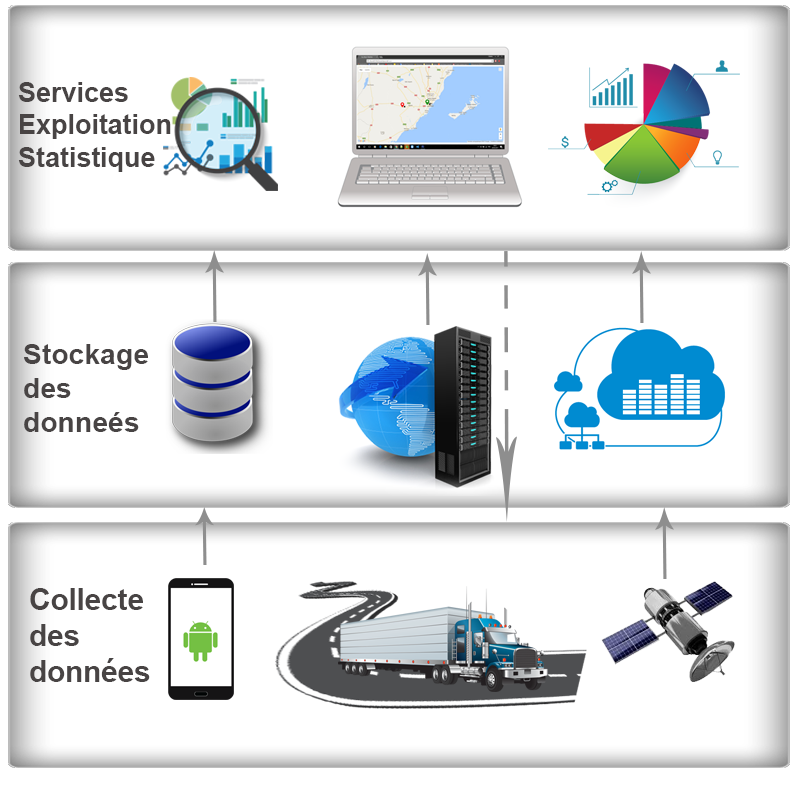
\includegraphics[width=1\textwidth]{citywatch-modules}
    \caption{Vue d'ensemble de la plateforme \textquote{City Watch}}
\label{fig:citywatch-modules}
\end{figure}

\section{Gestion du projet \textquote{City Watch}}

Chaque projet, surtout les projets innovant, doivent cibler une méthodologie du
travail adéquate pour organiser le travail. Parmi les méthodes actuelles, la
plus connue et répondue est la méthode ``Scrum''.

\subsection{Méthodologie agile Scrum}

Scrum est une méthode de gestion de projets dans laquelle des équipes
multifonctionnelles réalisent des produits de manière itérative et
incrémentale. Tout au long de cette méthode, le développement est défini,
d'une façon incrémentale, en cycles de travail appelés Sprints. Un sprint est
défini sous la forme d'un certain nombre de tâches à réaliser au cours d'une
itération. Cette dernière ne dure jamais plus que quatre semaines (deux
semaines la plupart du temps). Les itérations s'enchaînent l'une après l'autre
sans interruption. Les Sprints se terminent à une date spécifique. Ceux-ci ne
peuvent être prolongés même si le travail ne soit pas terminé. Généralement les
équipes Scrum choisissent une durée de Sprint et la maintiennent durant le
projet, jusqu'à ce qu'elles puissent encore augmenter leur productivité et
utiliser alors un cycle plus court. Au début de chaque Sprint, une équipe
multifonctionnelle sélectionne des tâches
(exigences du client) dans une liste priorisée. L'équipe s'accorde
collectivement sur une cible constituée de ce qu'elle pense pouvoir livrer à la
fin du Sprint. Aucune nouvelle tâche n'est ajoutée durant le Sprint. Chaque
jour, l'équipe se réunit brièvement afin de contrôler sa progression et ajuster
les prochaines étapes nécessaires à la finalisation du travail restant au sein
d'un Sprint. A la fin de chaque Sprint, une revue est organisée avec les
parties prenantes durant laquelle l'équipe montre ce qu'elle a réalisé. Le
feedback obtenu peut être pris en compte sur le Sprint suivant. Scrum insiste
sur la nécessité de livrer un produit opérationnel, testé et documenté à la fin
de chaque itération. La figure~\ref{fig:scrum-model} représente la méthode
agile Scrum.

\begin{figure}[H]
    \centering
    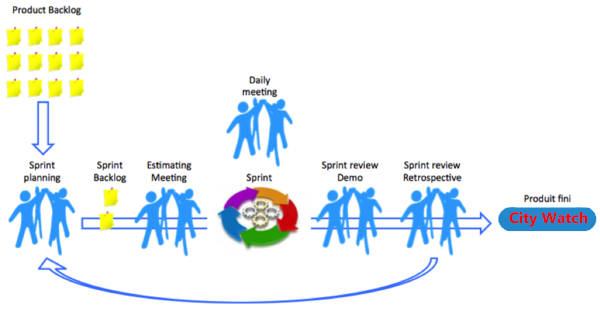
\includegraphics[width=.9\textwidth]{scrum-model}
    \caption{La méthode Génie Logiciel Scrum}
    \captionsource{\cite{scrum-model}, modifié}
\label{fig:scrum-model}
\end{figure}

L'application de la méthodologie Scrum dans notre projet \textquote{City Watch}
va être plus exploitée et détaillée dans le \autoref{sec:sprint0} ``Itération
0''. Ainsi, la réduction de cet rapport suivi un descriptif appliquant la
méthode Scrum donc le nom des chapitres suivants est basé sur le nom des
itérations Scrum.

\subsection{Justification du choix de la méthode agile Scrum}

Aujourd'hui, Les méthodes classiques présentent beaucoup d'inconvénients:

\begin{itemize}
    \item Parfois le client a du mal à exprimer son besoin. Un tel changement
        peut s'avérer coûteux d'autant la modification de certaines
        fonctionnalités dans le projet n'est pas tolérée dans la phase de
        développement. Ce que le nomme l'effet tunnel.
    \item Il est très difficile d'établir dès le début des paramètres stricts
        et clairs qui répondent aux attentes du client.
\end{itemize}

À fin d'éviter ces problèmes, Les caractéristiques de la méthode Scrum offre
des avantages considérables pour gérer ces problèmes:

\begin{description}
    \item [Personnel engagé] L'une des caractéristiques de Scrum, c'est que le
        personnel participe activement à la définition des activités et des
        horaires, de sorte que le degré d'engagement et la motivation sont plus
        élevés.
    \item [Meilleur vue d'ensemble du projet] Avec Scrum, les projets
        précédemment vus dans leur globalité et de façon homogène uniquement
        par les gestionnaires de projets sont désormais accessibles à tous les
        membres de l'équipe de livraison.
    \item [Réduction des bugs] La méthode Scrum privilégie la qualité et la
        fonctionnalité des développements. Le nombre de bugs et de reprises est
        ainsi réduit.
    \item [Mise à jour des priorités] Au début, le client ignore toute la
        portée de l'application, ainsi que la façon dont cela pourrait changer
        avec le temps. Grâce à Scrum, le client bénéficie d'une flexibilité au
        niveau de la définition, de l'évolution des priorités et des séquences
        d'activités.
    \item [Qualité du produit mise en avant] La méthode Scrum se concentre
        davantage sur la fourniture d'un service de valeur au client plutôt que
        sur une date limite fixée.
\end{description}

La nature d'itérations du Scrum et l'engagement des tous les membres concernés
par le projet permettent l'affinement continuel de quatre variables du
projet, nommées \textquote{Project Diamond} et présentés par la
figure~\ref{fig:project-diamond}:

\begin{description}
    \item [Fonctionnalités] Les cas d'utilisations demandés par le client.
    \item [Ressources] Budget fourni par le client.
    \item [Qualité] Qualité du code à maintenir par l'équipe.
    \item [Temps] Estimation par l'équipe pour la réalisation du code.
\end{description}

\begin{figure}[H]
    \centering
\tikzset{nodes={font=\ttfamily,fill=white}}
\begin{tikzpicture}[
        declare function={%
            f(\t)=90-\t*90;
            g(\t)=\t/2.5+1*\t/(0.1+\t);
            f2(\t)=-90-\t*90;
            g2(\t)=\t/2.5+0.8;
        },
        pos par/.style={%
            shift={({f2(#1)}:{g2(#1)})}
        },
        scale=0.68,
        every node/.style={transform shape},
    ]
    \draw[thick,->] (0,0) -- (0,4.7) node[above]{Fonctionnalités};
    \draw[thick,->] (0,0) -- (4.5,0) node[right]{Resources};
    \draw[thick,->] (0,0) -- (0,-4.5) node[below]{Qualité};
    \draw[thick,->] (0,0) -- (-4.5,0) node[left]{Temps};
    \draw[domain=0:8,variable=\t,smooth,samples=440,arrows={->[length=8]}]
         plot({f(\t)}:{g(\t)});
    \path node[pos par=0]{Itération 0}
          node[pos par=4]{Itération 1};
\end{tikzpicture}
\caption{Evolution du Projet Diamond en Scrum}
\label{fig:project-diamond}
\end{figure}


Scrum est la méthode idéale pour le cas d'une petite équipe et le fait d'avoir
un grand projet réparti entre cette équipe et aussi il est paraît la meilleure
solution pour répondre aux exigences du client et réduire la complexité
croissante de certains projets.

\section{Équipe \textquote{City Watch}}

\begin{figure}[!h]
    \centering
    
\includegraphics[width=.35\textwidth]{logo-citywatch}
    \caption{Logo du \textquote{City Watch}}
\label{fig:logo-citywatch}
\end{figure}

\textquote{City Watch} est une équipe de 8 membres qui a pris en main ce sujet
du zéro pour atteindre l'implantation du startup \textquote{City Watch}.
Durant la période du programme (5 mois), toute l'équipe a profité d'un ensemble
des formations:

\begin{description}
 \item [Hard Skills] Formations techniques et mentoring par un équipe des
     experts.
 \item [Soft Skills] Esprit d'équipe, flexibilité, adaptabilité et management.
\end{description}

L'équipe a lancé son site web \url{http://citywatch.factorycampus.net/public/}
et son propre logo représenté dans la figure~\ref{fig:logo-citywatch}.

Nous comme étions binôme de ce projet de fin d'étude, nous étions deux membres actifs faisant
partie dans l'équipe de \textquote{City Watch}. Nous avons participé activement
avec tous les autres membres de l'équipe à atteindre les buts tracés pour le
projet \textquote{City Watch}. Notre participation inclut toutes les parties du
projet, et l'essentiel de notre contribution va être présenté dans cette
manuscrit.

%\section{Applications similaires}

%Nous avons essayé d'étudier les applications similaires existantes dans le
%marché. Parmi les meilleurs applications les plus utilisées que nous avons
%trouvées sont Waze, Here WeGo.

%\begin{description}
%    \item [Waze] Une application de trafic et de navigation géographique. Il a
%        été fondé en 2006 par Ehud Shabatai et racheté par Google en Juin
%        2013~\cite{waze-google}. Waze a plus que 65,000,000 utilisateur active
%        par mois en 185 pays~\cite{waze-driverindex}.
%    \item [Here WeGo] (Anciennement Here Maps) Un logiciel de cartographie et
%        de navigation gratuit développé par HERE Global B.V., accessible à
%        partir d’un ordinateur, un téléphone ou d’une tablette. Il a été fondé
%        en 2014 par Nokia.
%\end{description}

\section*{Conclusion}
\addcontentsline{toc}{section}{Conclusion}

Le projet présent est effectué au sein de \textquote{Djagora Academy} au sein
de l'équipe \textquote{City Watch} qui vise à réaliser un système de collecte,
d'analyse et de valorisation des données tournantes autour du domaine de trafic
routier. Pour bien gérer ce projet, la méthodologie de gestion du projet Scrum
a été adoptée et ce pour minimiser les inconvénients connus aux méthodes de
gestions classiques.


\cleardoublepage
\chapter{Itérations}
\section[Itération 0: ( 2/20/2017 - 2/22/2017 )]{Itération~0:~\textup{\textto{(~2/20/2017~-~2/22/2017~)}}}

\subsection*{Introduction}

Avant de commencer la première itération du Scrum, une période de temps à été
consacrée pour préparer ce qui est nécessaire pour le lancement du projet dans
des bonnes conditions. Cette période est souvent nommée l'itération 0 du
projet. Elle est dédiée généralement à la recherche bibliographique, aux choix
technologiques et à la mise en place de l'environnement de développement.  Dans
cette itération nous définissons le Backlog général de notre projet, ainsi que
l'environnement du travail que nous avons besoin.

\subsection{Backlog général}

La première étape de la méthode Scrum consiste à préparer un carnet du produit
(Product Backlog) qui présente la liste des tâches à effectuer durant le
développement du projet qui sera répartie en des itérations. Le rôle du Product
Owner est important dans cette phase de développement parce qu'il devra faire
l'exercice de prioriser ses demandes selon des critères respectant la mission
et les objectifs de son produit. En précisant la valeur de priorité, il estime
l'impact et le retour sur investissement qu'aura chacun des items dans le
carnet du produit. Il y a donc effectivement eu un gros travail d'échanges et
discussions avec le client pour comprendre tout le cahier des charge initial,
C'est comme ça que le Backlog a été défini.

Les valeurs d'affaires sont définies comme suit :
\begin{description}[align=right,labelwidth=1cm]
    \item [1:] Définie une haute priorité, affectée pour les spécifications
        importantes, exigées pour le produit.
    \item [2:] Définie une priorité importante mais pas exigée.
    \item [3:] Définie une priorité moyenne ou parfois faible.
\end{description}

La figure~\ref{fig:product-backlog} présente une version simplifiée du Product
Backlog complète des 3 premières itérations. Nous représentons notre
participation par les cercles du texte souligné.

\usetikzlibrary{mindmap,shadows}
\newcommand*{\info}[4][16.3]{%
  \node [ annotation, #3, scale=0.65, text width = #1em,
          inner sep = 2mm ] at (#2) {%
  \list{$\bullet$}{\topsep=0pt\itemsep=0pt\parsep=0pt
    \parskip=0pt\labelwidth=8pt\leftmargin=8pt
    \itemindent=0pt\labelsep=2pt}%
    #4
  \endlist
  };
}
\begin{figure}[htbp]
%\usepackage{dtklogos}
\hspace{-9ex}
\begin{tikzpicture}[every annotation/.style={draw, fill=white, font=\Large}]
    \renewcommand{\href}[2]{#2}

    \path[mindmap,
          concept color=black!40,
          text=white,
          every node/.style={
              concept,
              circular drop shadow,
              execute at begin node=\hskip0pt,
          },
          %grow cyclic,
          root/.style={
              concept color=black!40,
              fill=white, line width=1ex, text=black,
              font=\footnotesize\bfseries,
              text width=7em},
          level 1 concept/.append style={
              font=\normalsize\bfseries,
              sibling angle=50,
              text width=7.7em,
              level distance=12.5em,
              inner sep=0pt},
          level 2 concept/.append style={
              font=\footnotesize\bfseries,
              level distance=8em},
          ours/.append style = {
              line width=0.5ex,
              concept color = black,
          }
    ]

    node[root] {Platforme CityWatch} [clockwise from=0]

    child[concept color=blue!70] {
        node {\ul{Gestions des Rapports}} [clockwise from=50]
        child { node { \ul{Consultation} } }
        child { node { \ul{D\'eclaration} } }
    }
    child[concept color=green!40!black] {
        node[concept] {\ul{Information Routi\`ere}} [clockwise from=30]
        child { node[concept] {\ul{Secousses}} }
        child { node[concept] {\ul{Ralentisseurs}}}
        child { node[concept] {Embouteillage}}
    }
    child[concept color=blue] {
        node[concept] {\ul{Itin\'eraire}} [clockwise from=305]
        child { node[concept] {\ul{Localisation instantan\'e}} }
        child { node[concept] {\ul{Projection du Trajectoire}} }
        child { node[concept] {\ul{Historie des Trajectoires}} }
    }
    child[concept color=red!60!black] {
        node[concept] {Assistance} [clockwise from=235]
        child { node[concept] {Alerte des secousses} }
        child { node[concept] {Alerte des ralentisseurs} }
    }
    child[concept color=orange] {
        node[concept] {\ul{Tableau de Bord}} [counterclockwise from=100]
        child { node[concept] {\ul{Carte en Temps R\'eel}}}
        child { node[concept] {\ul{Authentification}} }
        child { node[concept] {\ul{Filtrages}} }
    }
    child[concept color=yellow!60!black] {
        node[concept] (Blogs) {\ul{Analyse et Visualisation}} [clockwise from=135]
        child { node[concept] {Visualisation des données}}
        child { node[concept] {\ul{Tableau du bord interactive}}}
    }
    child[concept color=red] {
        node[concept] {Information Réseau} [clockwise from=110]
        child { node[concept] {Signal Réseau} }
        child { node[concept] {Génération Réseau} }
        child { node[concept] {Opérateur Réseau} }
    };
\end{tikzpicture}
\caption{Objective du produit}
\label{fig:product-backlog}
\end{figure}


Le tableau~\ref{tab:product-backlog} représente la liste plus détaillé des cas
d'utilisations que nous allons implémentés pendant les 3 premières itérations.
Ils suivent la forme:
\begin{displayquote}
    En tant que \textbf{X}, je peux \textbf{Y} Afin d'\textbf{Z}.
\end{displayquote}
ou aussi la forme:
\begin{displayquote}
    En tant que \textbf{X}, je veux qu'il soit possible de \textbf{Y} pour
    \textbf{Z}.
\end{displayquote}

Dans notre liste des cas d'utilisation, l'acteur initiateur (\textbf{X}) est
toujours l'utilisateur.

\Needspace{5\baselineskip}
\begin{center}
    \footnotesize
    \setlength\LTleft{-20pt}
    \begin{longtable}{| l | p{3.5cm} | p{5.5cm} | p{5cm} | l |}
 \caption{Backlog du Produit}
 \label{tab:product-backlog} \\

 \hline
 \textbf{ID} & \textbf{Cas d'utilisation} & \textbf{Je veux qu'il soit possible de} & \textbf{Pour} & \textbf{Priorité} \\ \hline
 \endhead

 \hline \multicolumn{5}{|r|}{{Continué en page suivante$\dotsc$}} \\ \hline
 \endfoot

 \hline \hline
 \endlastfoot

\hline
%1 & Gestion du Trajectoire & démarrer le localisation & Avoir un feedback dans l'application et sur le site web & 1 \\ \cline{3-5}
%  &                        & arrêter le localisation & Avoir un feedback dans l'application & 1 \\ \hline
%2 & Gestion de Rapports    & choisir entre une variété de problèmes à déclarer depuis l'application & Avoir un feedback sur le site web & 1 \\ \cline{3-5}
%  &                        & choisir l'emplacement du problème à déclarer dans une carte & Avoir un feedback sur le site web & 1 \\ \cline{3-5}
%  &                        & ajouter une description ou une image au problème & Avoir un feedback sur le site web & 2 \\ \hline
%3 & Consulter la carte     & consulter la carte depuis l'application & Voir la carte dans l'application & 2 \\ \hline
%4 & Compte                 & consulter le site web sans avoir un compte & Consulter le site web avec un minimum d'informations & 1 \\ \cline{3-5}
%  &                        & créer un compte & Avoir un compte personnel & 2 \\ \hline
%5 & Groupement des rapports& voir les rapports en groupe lors d'un zoom out & Avoir une vision globale sur le nombre des rapports & 1 \\ \hline
%6 & Déclarer un rapport    & déclarer un rapport à partir du site web & Avoir accès à une page rapport comme celle de l'application & 1 \\ \hline
% \hline \ldots & \ldots & \ldots & \ldots & \ldots \\ \hline

%
1 & Gestion du Trajectoire & Activer le localisation & Enregistrer le trajectoire & 1 \\ \cline{3-5}
&                          & Consulter le dashboard  & Afficher le trajectoire instantané & 1 \\ \cline{3-5}
&                          & Filtrer le trajectoire  & Consulter l'histoire des trajectoires & 2 \\ \hline
2 & Gestion des Rapports   & Déclarer un rapport depuis le site & Avoir un rapport dans la carte & 1 \\ \cline{3-5}
&                          & Choisir un emplacement & Afficher et filtrer par catégorie & 1 \\ \cline{3-5}
&                          & Ajouter une image et commentaire & Enrichir le rapport & 1 \\ \cline{3-5}
&                          & Accéder à formulaire depuis l'application mobile & rapporter instantané et facilement & 2 \\ \cline{3-5}
&                          & Activer/Désactiver le groupement des marqueurs & Avoir une vision sur le nombre des rapports plus claire & 3 \\ \hline
3 & Tableau de bord (Dashboard) & Consulter le dashboard & Visualiser diffèrent type de données comme marqueurs et zones & 1 \\ \cline{3-5}
&                               & Manipuler la légende   & Filtrer les données affichés & 1 \\ \hline
4 & Comptes                & Créer un compte & Pouvoir enregistrer des données personnels (trajectoire) & 3 \\ \cline{3-5}
&                          & Se connecter & Accéder au données routières privées (trajectoire) & 3 \\ \cline{3-5}
&                          & Visiter le dashboard sans compte & Consulter une version minimale des fonctionnalités & 3 \\
\hline
\end{longtable}
\end{center}

\subsection{Préparation de l'environnement du travail}

\subsubsection{Environnement logiciel}

La réalisation de ce projet nécessite l'ensemble de ces logiciels et
bibliothèques que nous allons sites :

\paragraph{Android}

On a choisi du supporter le système Android comme notre première plateforme. Ce
choix était basé sur différents aspects:
\begin{itemize}
    \item La part de marché des smartphones et tablettes Android.
    \item L'ouverture de la plateforme, et l'accessibilité aux différentes
        fonctionnalités et aux outils de développements.
    \item Android Auto, Android Wear, Android Things\ldots
\end{itemize}

Android Studio\footnote{Android Studio v2.3} était le choix naturel pour le
développement d'application grâce au support officiel du Google et les
fonctionnalités héritées de l'ide IntelliJ IDEA de JetBrains comme un
concepteur d’interface utilisateur pour des résolutions variées simultanément,
débogueur, \ldots

%\subparagraph{Android studio}
%est un environnement de développement pour développer des applications Android.
%Il est basé sur IntelliJ IDEA.\\ Android studio permet principalement d'éditer
%les fichiers Java et les fichiers de configuration d'une application Android.Il
%propose entre autres des outils pour gérer le développement d'applications
%multilingues et permet de visualiser la mise en page des écrans sur des écrans
%de résolutions variées simultanément

\paragraph{PHP}
En se basant sur les conseils du Product Owner et aux limites d'environnement
de développement dont le serveur supporte seulement PHP, on a choisi la langue
de programmation PHP\footnote{PHP 7.0}.

Les points fort de la langue PHP:
\begin{itemize}
    \item Une langue très répondu dans le développement Web, Elle a une
        grande communauté des développeurs.
    \item Une grande liste des outils de développement incluant les
        gestionnaires des dépendances (Composer, Phar), outils des tests
        unitaires (PHPUnit), générateurs du documentation (PHPDoc, Sami),
        débogueurs (Xdebug), analyseurs du code et analyseurs statiques
        (php\_CodeSniffer, PHPLint), outils d'automatisation (Phing) and
        multiple IDEs.
    \item Multiple bibliotheques et frameworks pour différent type des projets.
\end{itemize}

Les points faibles de la langue PHP:
\begin{itemize}
    \item Gestion d'erreurs très souple par défaut même si les erreurs sont
        fatales.
    \item Manque d'un paradigme unique dans l'architecture de la langue (le
        choix du syntaxe et du noms des fonctions)
\end{itemize}

L'ide choisie pour le développement PHP est PHPStorm\footnote{PHPStorm 2017.1},
un IDE multiplatforme de JetBrains. Il regroupe sous une interface conviviale
un éditeur de texte avancé et intelligent, un interpréteur et un
débogueur\ldots. Vim a été aussi utilisé avec un ensemble des extensions pour
enrichir ses fonctionnalités.

%\paragraph{Composer}
%
%Le logiciel Composer est un gestionnaire de dépendances sous licence libre
%écrit en PHP\@. Il permet à ses utilisateurs de déclarer et d'installer les
%bibliothèques dont le projet principal a besoin.

\paragraph{Technologies du Web}

Les technologies Web modernes nous ont permis de créer une application web
interactive et dynamique rapidement et aisément sans besoin d'un backend pour
générer le contenu.

\begin{description}
    \item [HTML 5.1] On a utilisé les tags sémantique, les nouveaux types et
        attributes de validations des entrés du formulaire et les nouveautés
        des api Web comme l'api DOM et l'api de localisation.
    \item [CSS 3] Ou plus précisément les modules stabilisés du CSS niveau 3.
        \TODO{used indirectly throw Bootstrap 3/4}
    \item [ECMAScript 2016\textregistered] Ou encore JavaScript edition 7
        définit définit dans la spécification ECMA-262 \cite{ECMA262}. On a
        utilisé le programmation POO, la programmation asynchrone (Promise) et
        des autres nouveautés de syntaxe.
\end{description}

L'utilisation de ces dernières mise à jours des standards du web a causé que
notre application web est supporté par seulement les dernières versions des
navigateurs principales\footnote{Firefox v45+ (sans support d'input de type
date), Google Chrome v50+, Edge v14+, Sfari 10+ (sans support d'input de type
date), Opera 37}. Le support des autres anciennes versions et des autres
navigateurs était possible en demande à travers les transcompilateurs du
ECMAScript 2016+ à ECMAScript 5.1 comme Babel ou Traceur même si il n'était pas
une priorité pendant notre phase de développement. Quelques fonctionnalités de
ECMAScript 2016 n'étaient pas utilisées car elles ne sont pas encore
implémentées par aucun des navigateurs principales comme les Modules.

\subsubsection{environnements matériels}

Pour le développement de ce projet, il était demandé d'avoir :
\begin{itemize}
 \item Serveur Local pour les tests
     \begin{itemize}
         \item Windows 10
         \item Wamp 3.0
         \item Apache 2.4
         \item PHP 7.0
         \item MySQL 5.7
     \end{itemize}
 \item Serveur de production:
     \begin{itemize}
      \item Linux
      \item Accès FTP
      \item Apache 2.4
      \item PHP 7.0
      \item MySQL 5.5
     \end{itemize}
\end{itemize}
\subsection{Étude de l'existence de notre projet}
L'idée de notre projet n'est pas usuelle comme les autres, tout simplement est
une idée de startup que nous allons l'exploité dans le marché. C'est pour ce là
que nous étudions les applications similaires pour avoir notre position.
\subsubsection{Waze}
\paragraph{Caractéristiques communes}
\begin{itemize}
    \item Détection de d'embouteillages.
    \item Les utilisateurs peuvent utiliser leur téléphone pour contourner
        passivement le trafic et d'autres données routières. Ils peuvent
        également jouer un rôle plus actif en partageant les rapports routiers
        sur les accidents, les pièges policiers ou tout autre danger en cours
        de route.
    \item Informé l'utilisateur en avance des incidents trouvé dans la route
        suivi.
\end{itemize}

\subsection{Conclusion}

L'itération 0 nous à permis de préparer le terrain pour une bonne entame de
développement. Indépendamment la mise en place des environnement de travail et
les formations que nous avons suivi sur les technologies.  Pendant cette
itération nous avons élaborer le carnet de notre projet avec la collaboration
du Product Owner.

\section[Itération~1:~(~2/22/2017~-~3/5/2017~)]{Itération~1:~\textup{\textto{(~2/22/2017~-~3/5/2017~)}}}

\subsection{Introduction}

La méthodologie Scrum consiste à développer le produit incrémentalement, en
effet chaque itération résulte un prototype ayant des fonctionnalité du produit
demandé livrable. Le développement de ces fonctionnalité est en parallèle avec
d'autre fonctionnalité puisque l'équipe avance dans le même niveaux.

\subsection{Objectif de l'itération}

L'objectif de cette itération vise deux environnement:

\begin{description}
    \item [Mobile] Créer une première version d'application mobile permettant
        de localiser des utilisateurs selon leur position actuelle.
    \item [Web] Projeter instantanément la position de l'utilisateur sur une
        carte map avec son état (activé ou désactivé)
\end{description}

\begin{figure}[htbp]
    \centering
    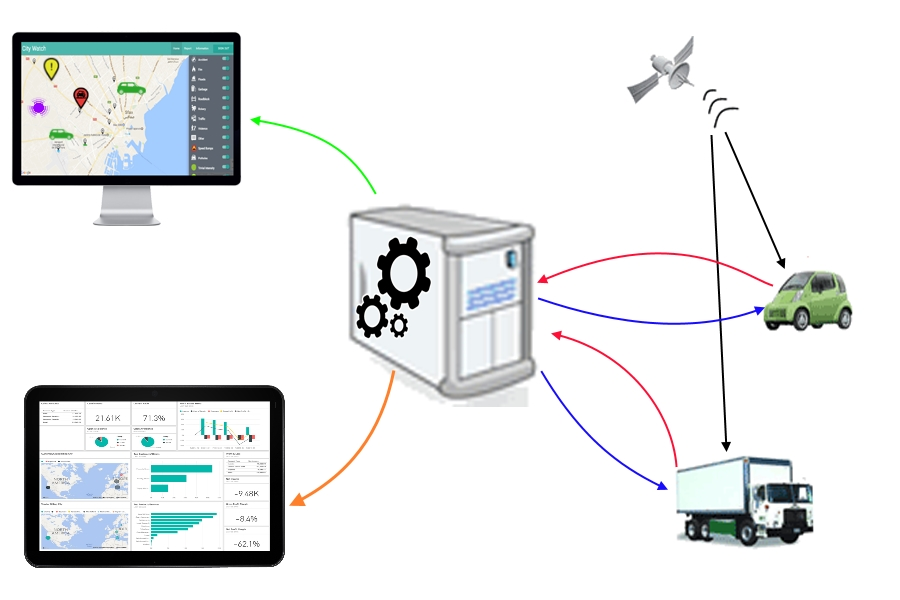
\includegraphics[width=0.8\textwidth]{citywatch-architecture}
    \caption[Flux des information Géographiques en CityWatch]
    {Flux des informations Géographiques dans le système de localisation}
    \captionsource{}{http://masterhaniff.blogspot.com/2014/11/vehicle-tracking-system.html}
    \label{fig:citywatch-architecture}
\end{figure}

%L'objectif de cette itération est d'étudier notre Serveur, de générer notre
%modèle, de réaliser la page Web (dashboard) et développer les vues nécessaires
%pour permettre à l'utilisateur de consulter la dernière position du véhicule
%selon les spécifications du Backlog.

%Une fois la première ébauche du Backlog est réalisée, le Product Owner peut
%découper les spécifications de haut niveau vers des spécifications plus
%raffinées. Dès lors, nous passons à la planification d'une itération. Il est
%important de rappeler que les premières spécifications du Backlog doivent être:

%\begin{itemize}
%    \item assez précise pour être estimée par l'équipe.
%    \item assez petite pour être développée et testée durant une itération.
%\end{itemize}

%Ayant une bonne idée sur le produit ainsi que l'objectif à atteindre, l'équipe
%et le Product Owner peuvent passer à l'élaboration des itérations. Dans notre
%projet \textquote{Plateforme CityWatch}, la durée d'une itération est fixée à
%trois semaines. Dans cette section, nous décrivons le déroulement de la
%première itération. Une itération commence par sa planification et finit par
%être revue avec le \textquote{Product Owner}.

\subsection{Planification de l'itération}

Dans le but de définir le périmètre fonctionnel de l'itération 1 et faire sa
planification, tous les membres de l'équipe ont participé à un réunion avec le
Scrum Master et le Product Owner pour définir le backlog du sprint.

La planification de l'itération représente une étape importante dans la vie de
l'itération parce que au cours du planification, on divise l'itération a
plusieurs tâches pour mieux atteindre le résultats attendu à la fin de
l'itération.

Dans cette première itération, on a décidé de diviser cette itération en trois
grandes parties:

\begin{enumerate}
    \item Une partie consacrée pour la création de la base de donnée et les
        services web.
    \item Une partie consacré pour la réalisation de la page d'accueil.
    \item Une partie qui répond aux besoins des autres tâches de cette
        itérations.
\end{enumerate}

\subsubsection{Backlog de l'Itération}

Les tâches à réaliser peuvent \HTODO{être soient}{contenir?} des tâches de
recherche, de documentation, de conception, de développement ou bien
d'installation, de tests, d'intégration, etc\ldots. Il est recommandé lors de
la planification de la liste des tâches de bien les détailler. Une tâche ne
doit pas inclure d'autres tâches. Ceci permet de bien cerner le travail
demandé.

\begin{center}
    \footnotesize
    \begin{longtable}{| p{1cm} | p{5cm} | p{7cm} | p{1cm} |}
        \caption{Backlog de l'itération 1}
        \label{tab:sprint1-backlog} \\

        \hline
        \textbf{Réf} & \textbf{Spécification} & \textbf{Description} & \textbf{Priorité} \\ \hline
        \endhead

        \hline \multicolumn{4}{|r|}{{Continué en page suivante$\dotsc$}} \\ \hline
        \endfoot

        \hline \hline
        \endlastfoot

        \hline
1.1 & Présentation et Configuration SVN & Présenter SVN, installer le serveur SVN et créer les répertoires & 1 \\ \hline
1.2 & Recherche sur les Services Web & Présenter les différentes Solutions des services web et choisir la meilleur solution & 1 \\ \hline
1.3 & Implémenter service Save Position & Enregistrement les coordonnées requis dans la base de données & 2 \\ \hline
1.4 & Implémenter la consommation du service Save Position & Coordonnées enregistrés instantané et continuellement dans la BD & 1 \\ \hline
1.5 & Recherche sur les spécifications de la plateforme Android & Présenter le modèle de développement Android et choisir le SDK optimale & 1 \\ \hline
1.6 & Création squelette de l'application mobile & Application fonctionnel (sans les fonctions de localisation) avec l'IHM nécessaire et l'intégration au SVN & 1 \\ \hline
1.7 & Implémenter service Get Last Position & Le serveur retourne les dernières coordonnées requis & 1 \\ \hline
1.8 & Rectification service Save Positon & Support multiple périphériques et enregistrer la date d'envoyé & 2 \\ \hline
1.9 & Rectification service Get Last Position & Retourné la position du périphérique et la date du dernier modification & 2 \\ \hline
1.10 & Affiche Multiple marqueurs & Afficher dernière position de chaque périphérique dans la carte & 2 \\ \hline
1.11 & Affiche état du périphérique & Afficher si le périphérique est en ligne ou hors ligne & 3 \\ \hline
    \end{longtable}
\end{center}

\subsubsection{Estimation de la Première Itération}

Nous avons fixé la période d'une itération à 3 semaine. Dans le
tableau~\ref{tab:sprint1-capacity}, nous présentons une estimation du nombre
d'heures pendant lesquelles nous nous engageons à travailler.

\begin{table}[htbp]
    \centering
    \begin{tabular}{| c | c | c | c |}
        \hline
        \textbf{Membre} & \textbf{Nombre d'heures par jour} & \textbf{Nombre de jours présent} & \textbf{Total en heures} \\ \hline
        \hline

Moez & 6 & 10 & 60\\ \hline
Rihab & 6 & 10 & 60 \\ \hline
\multicolumn{2}{c|}{} & \textbf{Total} & 120 \\ \cline{3-4}
    \end{tabular}
    \caption{Nombre d'heures de travail estimé de l'itération 1}
    \label{tab:sprint1-capacity}
\end{table}

Tout les membres de l'équipe font ensuite l'estimation de temps (en point
d'histoire d'utilisateur) de chaque tache avec le poker de planning. Les
estimations utilisés sont $\frac{1}{2}$, $1$, $2$, $3$, $5$, $8$, $13$. Les
taches peuvent aussi être assignées aux plus qu'un seul membres.

Le tableau~\ref{tab:sprint1-estimation} représente les estimations de nos
taches en heures ($x2$ signifie que la tache était assigné à deux membres) et
le membre à qui était assignée la tache.

\begin{center}
    \begin{longtable}{| l | l | l |}
        \caption{Nombre d'heures estimé pour la réalisation des taches}
        \label{tab:sprint1-estimation} \\

        \hline
        \textbf{Spécification} & \textbf{Membre} & \textbf{Heures} \\ \hline
        \endhead

        \hline \multicolumn{3}{|r|}{{Continué en page suivante$\dotsc$}} \\ \hline
        \endfoot

        \hline \hline
        \endlastfoot

        \hline
Présentation et Configuration SVN & Rihab & 5 x 2 \\ \hline
Recherche sur les Services Web & Moez & 13 x 2 \\ \hline
Implémenter service Save Position & Moez & 5 \\ \hline
Implémenter la consommation du service Save Position & Rihab & 5 x 2 \\ \hline
Recherche sur les spécifications de la plateforme Android & Rihab & 13 x 2 \\ \hline
Création squelette de l'application mobile & Rihab & 13 \\ \hline
Implémenter service Get Last Position & Moez & 5 \\ \hline
Rectification service Save Positon & Moez & 5 \\ \hline
Rectification service Get Last Position & Moez & 5 \\ \hline
Affiche Multiple marqueurs & Moez & 5 \\ \hline
Affiche état du périphérique & Rihab & 5 \\ \hline
    \end{longtable}
\end{center}

\subsubsection{Évolution du travail}

Au cours de l'itération, on a utilisé Excel et un tableau physique pour suivre
l'évolution des taches de chaque membre.

\clearpage % FIXME

Dans les figures~\ref{fig:sprint1-fig1},~\ref{fig:sprint1-fig2}
et~\ref{fig:sprint1-fig2}, on représente l'état du tableau des taches en jour
de distribution les taches, au milieu et à la fin de l'itération
respectivement. Les lignes colorés représentent nos taches. Les colonnes du
tableau sont:

\begin{description}
    \item [Who] L'allias du nom de chaque membres de l'équipe .

            \emph{Exemple }: RM signifie \textbf{R}ihab \textbf{M}ajdoub
    \item [À faire (Todo)] Les taches assignés au membres pour cette itération.
        L'échange des taches entre les membres est possible sur le supervision
        du Scrum Master.
    \item [Implémentation] La pourcentage de l'implémentation du tache de 0\%
        jusqu'à 100\%. Si le développeur a commencé l'implémentation d'une
        tache, il la déplace dans cette colonne et faire le mise à jour du
        pourcentage de l'implémentation à chaque jour pendant un court réunion
        nommée \textquote{Daily Scrum} pendant le, on discute l'évolution du
        travail et le plan du jour prochain.
    \item [Test/Intégration/Review] L'implémentation du tache est complete,
        elle est donc en phase d'évaluation et vérification de son
        fonctionnement si intégré dans le reste du système. Depuis la deuxième
        itération, au moins un autre membre doit revue le code pour à fin
        d'assurer la qualité du code, détecter et corriger les défauts le plus
        tôt possible.
    \item [Complete (Done)] La tache était implémentée et validée.
\end{description}

On a utilisé des différents couleurs pour différents types des taches:

\begin{description}
    \item [Rose] Les taches du développement d'interface web (Dashboard).
    \item [Verte] Les taches du développement mobile (l'application Android).
    \item [Jaune] Les taches du développement des services web et d'administration.
\end{description}

La liste des prochaines réunions est écrite dans le tableau aussi:

\begin{itemize}
    \item Présentations des recherches si la taches inclue une partie du
        recherche et présentation.
    \item Rendez-Vous avec des autres personnes concernés par le projet.
    \item Si un développeur est besoin d'aide ou de discusser un probleme
        recontré.
    \item Code Revue à la fin d'itération fait par tous les membres pour
        évaluer la qualité du code et détecter les défaults du conception et
        d'implementation.
\end{itemize}

\begin{figure}[htbp]
    \centering
    \caption{Évolution du travail}
    \begin{subfigure}{1\textwidth}
        \centering
        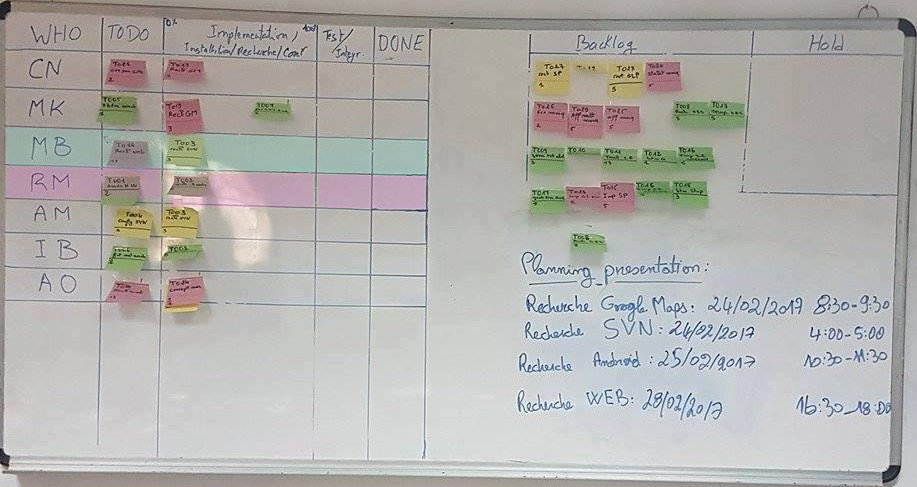
\includegraphics[width=0.8\textwidth]{sprint1-fig1}
        \caption{Distribution des taches de l'itération}
        \label{fig:sprint1-fig1}
    \end{subfigure}

    \begin{subfigure}{1\textwidth}
        \centering
        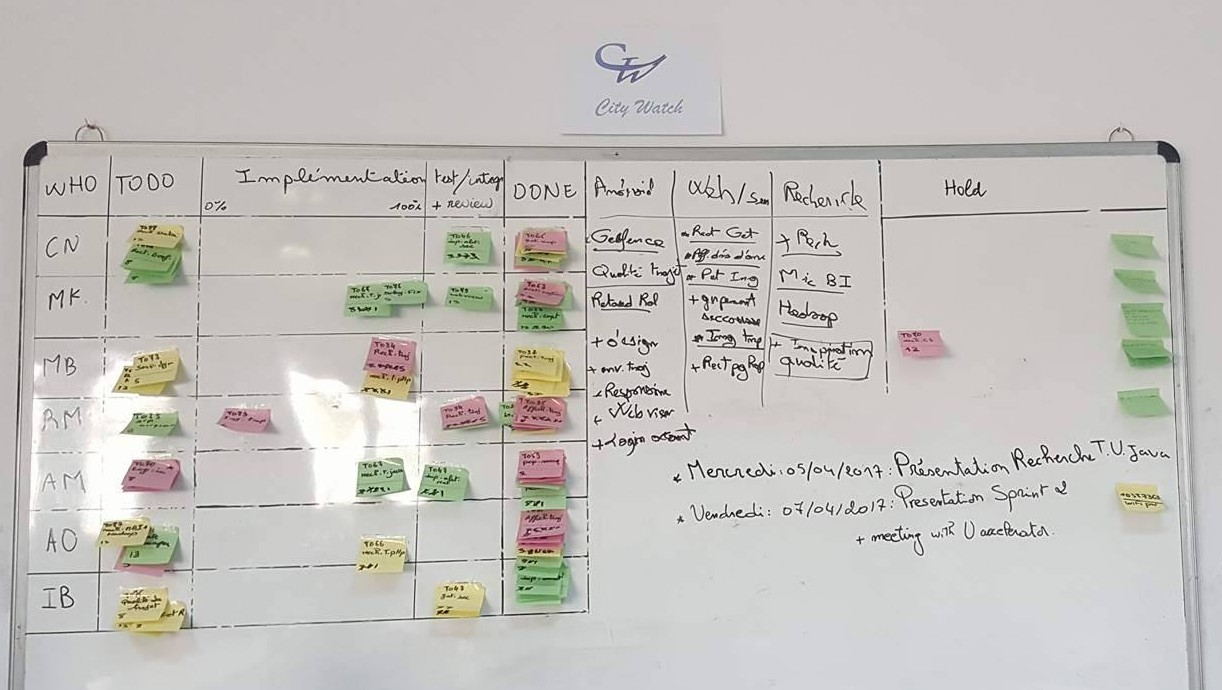
\includegraphics[width=0.8\textwidth]{sprint1-fig2}
        \caption{Au milieu d'itération}
        \label{fig:sprint1-fig2}
    \end{subfigure}

    \begin{subfigure}{1\textwidth}
        \centering
        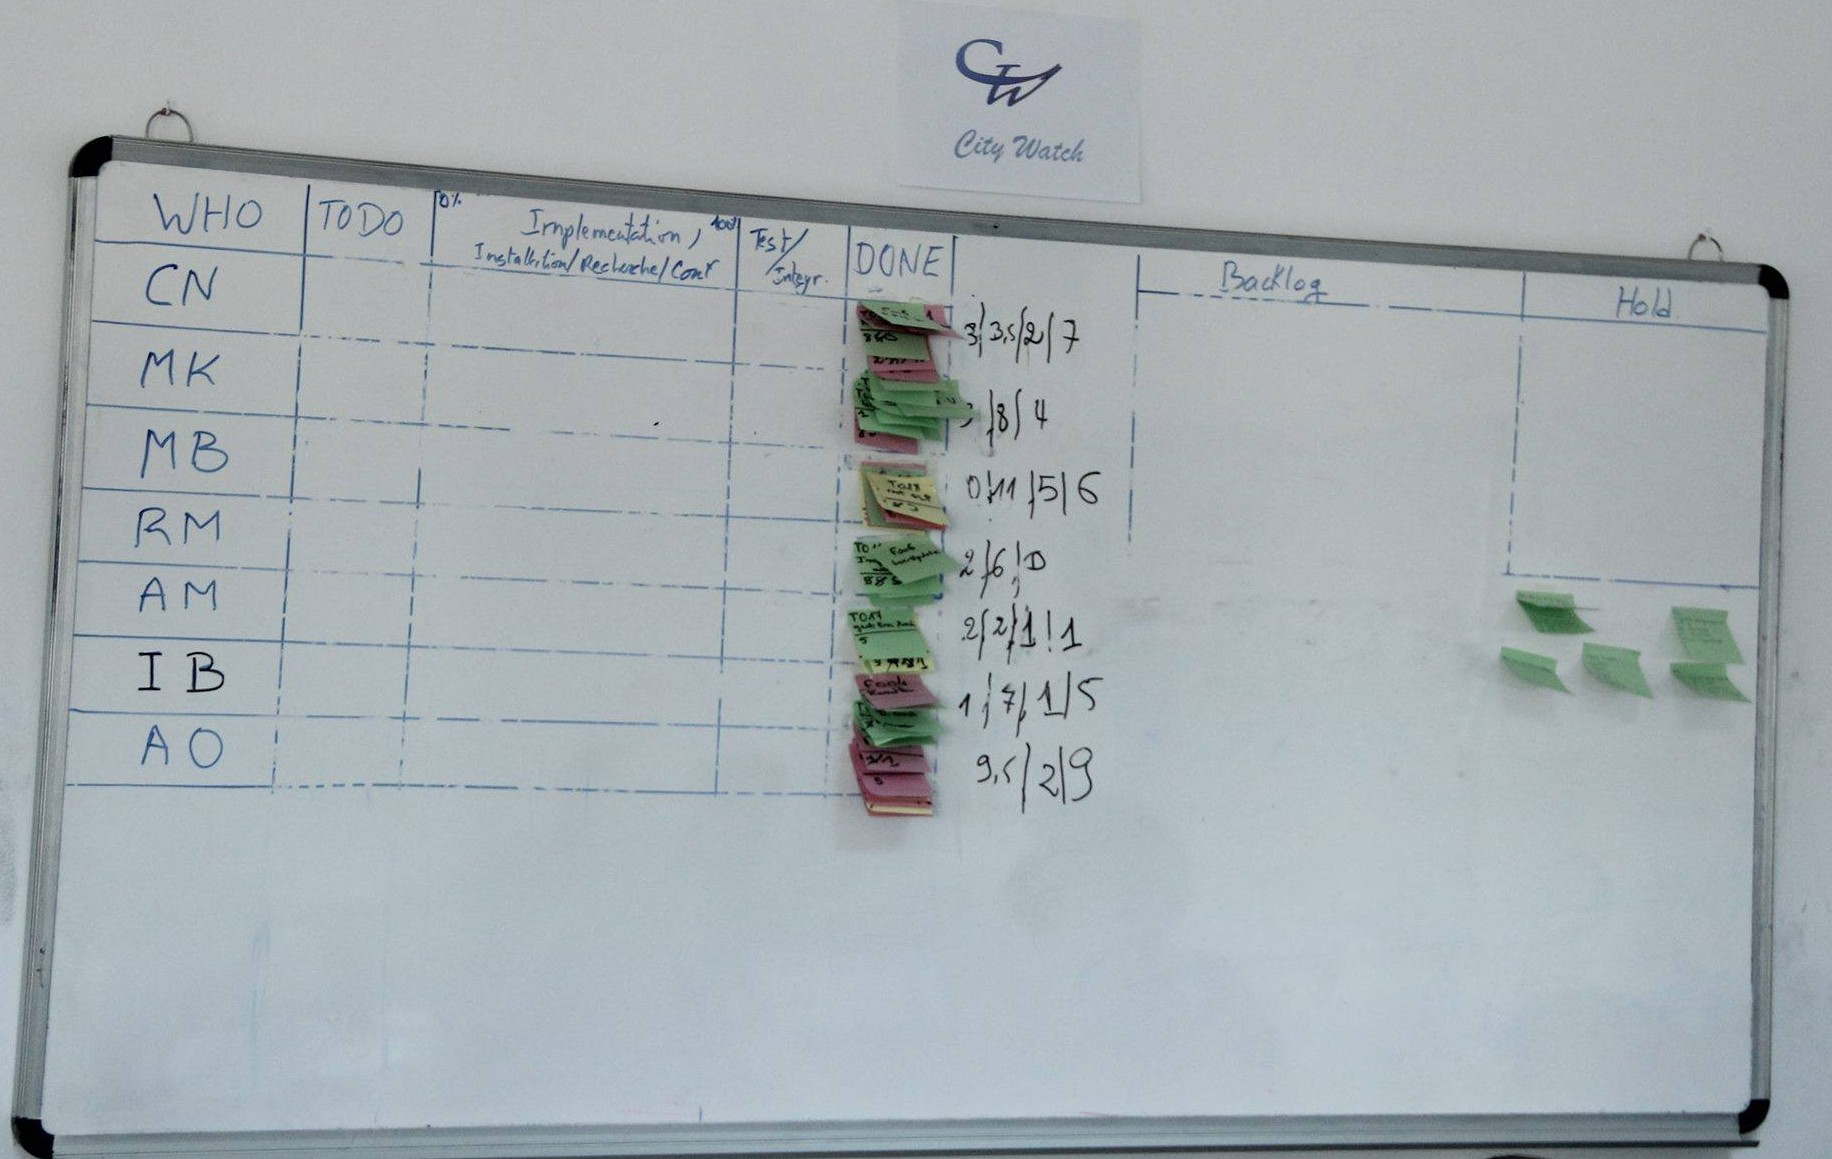
\includegraphics[width=0.8\textwidth]{sprint1-fig3}
        \caption{Au fin d'itération}
        \label{fig:sprint1-fig3}
    \end{subfigure}
\end{figure}
\clearpage

\subsection{Présentation des outils utilisés}

Le stage chez Djagora Academy nous a permis d'acquérir de nouvelles compétences
tant au niveau relationnel que technique. Pour bien entamer la réalisation de
la plateforme \textquote{City Watch}, nous avons suivi différentes formations
sur les outils et les technologies que nous venons de citer.

\subsubsection{Apache Subversion}

Les logiciels de gestion de versions \acrshort{VCS} nous permettent de
conserver la chronologie des modifications du source de code, ainsi récupérer
les version intermédiaires et les différences entre eux, et facilitent la
collaboration au développement. Les deux logiciels de gestion de versions les
plus répondus sont Git et Apache SVN\@.

\begin{description}
    \item [Git] Logiciel de gestion de versions distribué avec des branches
        légères. La récupération des versions précédentes et l'enregistrement
        des changements sont possibles sans besoin d'accès au dépôt distant car
        chaque développeur a une copie complète du dépôt. Le modèle Fork
        (Dupliquer), Commit (Modifier), Merge (Fusionner) a eu un grand succès
        dans les projets libres.
    \item [Apache SVN] Logiciel de gestion de versions centralisé. Il est connu
        pour sa simplicité comme il n'est pas un distinct entre un dépôt local
        vs. Dépôt distant, on faire juste une copie du dossier de travail d'une
        version précise. Les commandes sont simples:
        \begin{itemize}
            \item \verb|svn checkin| \ \ vs. \ \ \verb|git commit; git push|
            \item \verb|svn update| \ \ vs. \ \ \verb|git fetch; git rebase|
        \end{itemize}
        Le support du Windows est excellent surtout les outils graphiques. La
        plus tard des fonctionnalités du SVN nécessitent l'accès au dépôt
        (distant).
\end{description}

Apache SVN était choisi pour sa simplicité, sa bon support de Windows et pour
des exigences de spécification. \FIXME{improve sentence}

L'outil serveur choisi est VisualSVN Server pour sa simplicité d'installer et
de configurer et pour son support du Windows.

Les outils clients choisis sont:

\begin{itemize}
    \item TortoiseSVN pour l'intégration avec le système Windows.
    \item La commande de ligne \verb|svn| est utilisée en Linux.
    \item Le support de SVN est intégré au Android Studio et PHPStorm.
\end{itemize}

%Un logiciel de gestion de versions est un logiciel de gestion de configuration
%permettant de stocker des informations pour une ou plusieurs ressources
%informatiques permettant de récupérer toutes les versions intermédiaires des
%ressources, vainsi que les différences entre les versions.
%
%Apache Subversion (en abrégé SVN) est un logiciel de gestion de versions,
%distribué sous licence Apache et BSD\@.
%VisualSVN est un plug-in d'intégration de Subversion de qualité professionnelle.
%Les principaux avantages de VisualSVN sont les suivants:
%
%\begin{itemize}
%    \item Fiabilité imbattable: Visual Studio ne s'arrêtera jamais ni ne
%        s'arrêtera à cause de VisualSVN.
%    \item Intégration transparente: VisualSVN gère automatiquement les fichiers
%        ajoutés ou renommés et reflète ces opérations sur Subversion.
%    \item Statut en temps réel: VisualSVN suit attentivement et affiche toutes
%        les modifications apportées à votre copie de travail.
%    \item Courbe d'apprentissage courte: VisualSVN utilise les boîtes de
%        dialogue TortoiseSVN et fournit un assistant intelligent pour mettre
%        vos sources sous Subversion.
%\end{itemize}
%VisualSVN Server vous permet d'installer et de gérer facilement un serveur
%Subversion entièrement fonctionnel sur la plateforme Windows. Il est utile tant
%pour les petites entreprises que pour les entreprises.

\subsubsection{Android}

Android est un système d'exploitation conçu en 2007 \TODO{référence} par la
société Android, startup racheté par Google. Android est Open Source, ça veut
dire on peut lire le code de ce logiciel le modifier et le redistribuer.

\paragraph{Activity:}

Un utilisateur habile d'Android remarque que lors de l'exploitation d'une
application Android qu'il est en train de naviguer entre des fenêtres et
l'application ne afficher qu'une seule fenêtre à la fois ces fenêtre la sont
des activités on peut différencier ces activité a travers leur interface
graphique ceci s'applique sur la plupart des application Android car il y a des
applications qui contiennent pas d'activités. Un première idée qui nous frappe
la tète c'est que une activité est un conteneur d'élément graphique qui
constitue un interface graphique. Alors que ne non une activité n'est pas
seulement une interface graphique mais elle va établir les liens entre
l'interface graphique et la logique programma tique de plus l'activité contient
des informations sur le statut actuel de l'application qui s'appelle le
contexte ce contexte permet de faire la liaison entre le système Android et les
autres activités de l'application.

\subparagraph{États d'activités:}

Le système Android met en place un système priorités entre application par
exemple l'utilisateur est en train de naviguer sur internet et écouter de la
musique il reçois un appel comme l'application qui gère les appel est une
application plus prioritaire elle prend la du navigateur et le lecteur musique
pour que l'utilisateur puisse répondre a son appel. Si une application consomme
trop de ressources et peut bloquer le fonctionnement du système Android,
Android arrêtera cette application. Et aussi comme expliqué précédemment les
activités sont gères a partir d'un système de pile d'activités. D'où
l'apparition de plus d'un état qui sont centré sur l'activité.

On peut différencier ces états par leur visibilité:

\begin{itemize}
    \item État Active.
    \item État en Pause.
    \item État Arrêté.
\end{itemize}

\subparagraph{Cycle de vie d'une activité:}

Une activité n'a pas de contrôle sur son état. Son état change suivant un cycle
rythmique entre le système Android et les autres application (un système quasi
dépendant sur des priorités comme expliqué précédemment). La
figure~\ref{fig:android-activity} explique le cycle de vie d'une activité. Les
états sont représentés comme des méthodes parce que lors de la programmation,
ces états sont interroges par le nom de ces méthodes.

% Diagram of Android activity life cycle
% Author: Pavel Seda 
% Drawing part, node distance is 1.5 cm and every node
% is prefilled with white background
\begin{figure}[H]
 \centering
 \footnotesize

\begin{tikzpicture}[node distance=1.5cm,
    every node/.style={fill=white, font=\sffamily}, align=center]
  % Specification of nodes (position, etc.)
  \node (start)             [activityStarts]              {L'activité démarre};
  \node (onCreateBlock)     [process, below of=start]          {onCreate()};
  \node (onStartBlock)      [process, below of=onCreateBlock]   {onStart()};
  \node (onResumeBlock)     [process, below of=onStartBlock]   {onResume()};
  \node (activityRuns)      [activityRuns, below of=onResumeBlock]
                                                      {Activity is running};
  \node (onPauseBlock)      [process, below of=activityRuns, yshift=-1cm]
                                                                {onPause()};
  \node (onStopBlock)       [process, below of=onPauseBlock, yshift=-1cm]
                                                                 {onStop()};
  \node (onDestroyBlock)    [process, below of=onStopBlock, yshift=-1cm] 
                                                              {onDestroy()};
  \node (onRestartBlock)    [process, right of=onStartBlock, xshift=4cm]
                                                              {onRestart()};
  \node (ActivityEnds)      [startstop, left of=activityRuns, xshift=-4cm]
                                                        {Le processus est tué};
  \node (ActivityDestroyed) [startstop, below of=onDestroyBlock]
                                                    {l'activité est arrêtée};     
  % Specification of lines between nodes specified above
  % with aditional nodes for description 
  \draw[->]             (start) -- (onCreateBlock);
  \draw[->]     (onCreateBlock) -- (onStartBlock);
  \draw[->]      (onStartBlock) -- (onResumeBlock);
  \draw[->]     (onResumeBlock) -- (activityRuns);
  \draw[->]      (activityRuns) -- node[text width=4cm]
                                   {Une autre activité s'intercole devent notre activité} (onPauseBlock);
  \draw[->]      (onPauseBlock) -- node {Notre activité n'est plus visible}
                                   (onStopBlock);
  \draw[->]       (onStopBlock) -- node {L'activité est arrêtée par le système ou l'utilisateur} (onDestroyBlock);
  \draw[->]    (onRestartBlock) -- (onStartBlock);
  \draw[->]       (onStopBlock) -| node[yshift=1.25cm, text width=3cm]
                                   {L'activité revientsur le devant de la scène}
                                   (onRestartBlock);
  \draw[->]    (onDestroyBlock) -- (ActivityDestroyed);
  \draw[->]      (onPauseBlock) -| node(priorityXMemory)
                                   {Priorité élevée $\rightarrow$ plus mémoire}
                                   (ActivityEnds);
  \draw           (onStopBlock) -| (priorityXMemory);
  \draw[->]     (ActivityEnds)  |- node [yshift=-2cm, text width=3.1cm]
                                    {L'utilisateur retourne vers l'activité}
                                    (onCreateBlock);
  \draw[->] (onPauseBlock.east) -- ++(2.6,0) -- ++(0,2) -- ++(0,2) --
     node[xshift=1.2cm,yshift=-1.5cm, text width=2.5cm]
     {L'activité revient sur le devant de la scéne}(onResumeBlock.east);

  \end{tikzpicture}
  \caption{Diagramme de cycle de vie d'activite Android}
  \captionsource{Pavel Seda, \TeX example.net [Modifié]}{http://www.texample.net/tikz/examples/android/}
  \label{fig:android-activity}
\end{figure}


\subparagraph{Comment choisir le SDK optimale:}

Une SDK permet l'application de marcher sur la version Android visé et les
versions ultérieure il a noté de prendre en considération le taux des
utilisateurs visé par cette application. Aussi il faut travailler avec une SDK
digne de confidence qui n'a pas de problème ou bug qui peuvent bloquer ou
arrêter le fonctionnement de l'application le SDK choisi doit pouvoir supporter
les fonctionnalité offerte par l'application si on va utiliser une
fonctionnalité qui utilise les empreinte le SDK dont on a travailler
l'application doit supporter cette fonctionnalité lorsque le travail sur une
application est en groupe il est mieux que tous ce groupe utilise la même SDK
pour éviter tous problème de compatibilité et conflit entre versions de SDK
donc il faut choisir une SDK qui est populaire en utilisation et qui est
stable. Dans notre projet on va utiliser SDK 23 qui vise la version Android 6.0
ayant un taux d'utilisateur qui est 4.79 % des utilisateur d'Android notons que
cet SDK comporte la fonctionnalité d'Android les plus récentes et qui est
stable.

\subsubsection{Les Services Web}

Un service web est un protocole d'interface de communication et l'échange de
données entre applications et systèmes hétérogènes à distance en utilisant les
technologies Web (HTTP dans notre cas).

Pendant la conception de l'api du service de position, on a étudié les
différentes variantes des architectures des services web:

\begin{itemize}
    \item Orienté RPC (ex: XML-RPC, SOAP, JSON-RPC):
        \begin{itemize}
            \item Meilleur pour présenter des actions et commandes.
        \end{itemize}
    \item Orienté Ressources (ex: RESTful):
        \begin{itemize}
            \item Représenter les données sous formes des ressources.
            \item Utiliser les méthodes HTTP pour modifier/créer/lire/supprimer
                les données.
            \item Utiliser les paramètres d'URL pour passer des paramètres.
            \item Sans état.
            \item Meilleur pour modéliser un domaine et entités.
        \end{itemize}
\end{itemize}

On a choisi d'utiliser l'architecture RESTful comme notre API est mieux décri
comme ensemble des collections des données dont on peut effectuer avec des
actions CRUD\@.

\subsection{Mises des normes}

Les exigence de l'api RESTful sont:

\begin{description}
    \item [Performance] Le temps de réponse doit être en une durée raisonnable.
    \item [Multi-Utilisateurs] On doit avoir la possibilité de stocker et
        récupérer les positions des différents utilisateurs.
    \item [Stabilité] L'implémentation doit vérifier la structure des données
        reçus, la disponibilité des champs obligatoires et leurs formats.
    \item [Portabilité] Le système doit support la différence en zone du temps
        et en internalisation, format de présentation des données géologique et
        sa précision.
\end{description}


\subsection{Conception}

\begin{figure}[htbp]
    \centering
    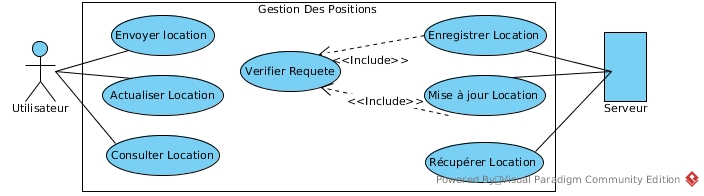
\includegraphics[width=1\textwidth]{sprint1-webservices-usecase}
    \caption{Diagramme de case d'utilisation du services web en itération 1}
    \label{fig:sprint1-webservices-usecase}
\end{figure}

%\begin{figure}[htbp]
%    \centering
%    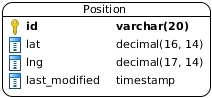
\includegraphics[width=0.45\textwidth]{sprint1-webservices-database}
%    \caption{Diagramme entité-association du service Position en itération 1}
%\end{figure}

\begin{figure}[htbp]
    \centering
    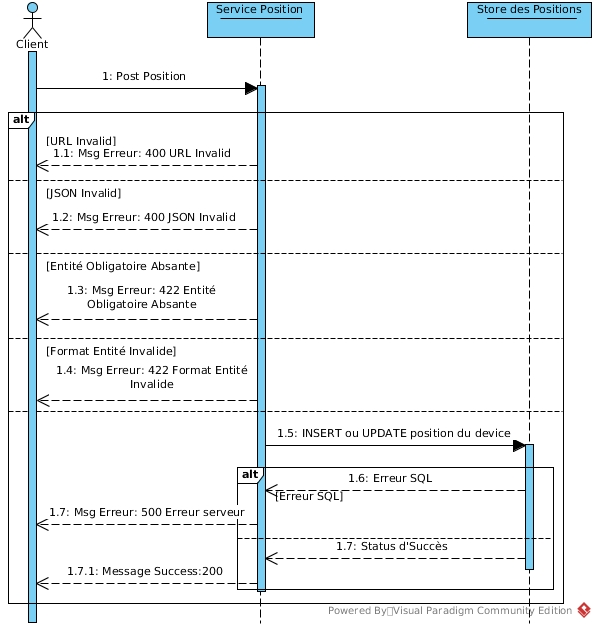
\includegraphics[width=1\textwidth]{sprint1-webservices-post-sequence}
    \caption{Diagramme de séquence du service Post Position en itération 1}
    \label{fig:sprint1-webservices-post-sequence}
\end{figure}

\begin{figure}[htbp]
    \centering
    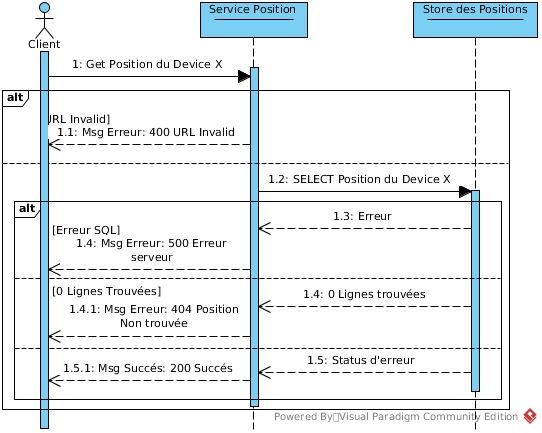
\includegraphics[width=1\textwidth]{sprint1-webservices-get-sequence}
    \caption{Diagramme de séquence du service Get Position en itération 1}
    \label{fig:sprint1-webservices-get-sequence}
\end{figure}

\subsection{Évaluation suivant les normes mise}

Avant de commencer le développement, on a fixé quelques règles à respecter pour
assurer la qualité du code.

\begin{itemize}
    \item Activer le mode strict du PHP et changer le mode de traitement des
        erreurs au déclenchement des exceptions si possible (PDO, \ldots).
        Activer le mode strict du JavaScript aussi.
    \item Utiliser des analyseurs statiques du code: PHP\_CodeSniffer, PHPLint
        et ESLint pour détecter les erreurs formelles de programmation ou de
        conception.
    \item Documenter chaque fonction, classe, constante et variable global. On
        a utilisé PHPDoc, apiDoc et JSDoc pour documenter le code PHP, l'api
        RESTful et le code JavaScript respectivement.
    \item Ecrire les tests unitaires pour les fonctions et les classes selon la
        technique \acrshort{TDD}. On a autorisé l'ecrire des tests unitaires
        aprés le développement du code. Les outils utilisés sont PHPUnit pour
        PHP et Mocha/Chai pour JavaScript. \TODO{Move to sp2}
\end{itemize}

Dans 1\ier{} phase, on a implémenté les méthodes POST et GET du ressource
Position. L'architecture résultante est documentée dans
l'annexe~\ref{appendix:sprint1-position-post-doc}
et~\ref{appendix:sprint1-position-get-doc}.

On a essayé d'adresser les différents les mises des normes spécifiés;

\subsubsection{Performance}

On a minimisé la dépendance en bibliothèques externes et extensions PHP\@. De
plus, Le nombre des requêtes SQL ont étés minimisés à une seule requêtes pour
chaque méthode du notre service web.

\subsubsection{Multi-Utilisateurs}

Les positions à enregistrer doivent contenus un id qui doit être utilisé aussi
pour retirer la dernière position. On a utilisé diffèrent identificateur pour
chaque périphériques basé sur le MAC du phone.

\subsubsection{Portabilité}

On a utilisé la format standardisée JSON~\cite{ECMA-404} pour le transfert de
données ce qui assure la portabilité des représentations des différents types
des données (nombres, booléens, strings, \ldots) indépendant du
l'internationalisation (séparateur décimal, \verb|true| vs. \verb|True| vs.
\verb|vrai| vs. \verb|yes| vs. \verb|y|, \ldots).

Pour le représentation des dates dans le content du requêtes HTTP, on a utilisé
la format RFC3339~\cite{RFC3339} (basé sur ISO8601~\cite{ISO8601} pour
l'utilisation dans les protocols du Web) avec UTC comme la défaut zone du
temps, ex: \verb|2005-08-15T15:52:01Z|.

Pour les en-têtes du requêtes HTTP, la format de représentation des dates est
RFC1123~\cite{RFC1123}, ex: \verb|Mon, 15 Aug 2005 15:52:01 +0000|.

La format du présentation des positions géologique (latitude et longitude)
choisie est la même représentation des nombres en JSON avec une précision
jusqu'à 14 chiffres après le séparateur décimal. Les valeurs envoyés doivent
respecte l'intervalle des diffèrent entités géologiques ($latitude \in [-90,
90]$, $longitude \in [-180, 180]$)

\subsubsection{Stabilité}

Pour assuré la stabilité d'un service web, on doit vérifier la validité de
contenu reçu même si envoyé depuis un source de confiance avant de les
utiliser. La vérification inclue le test de disponibilité des entités
obligatoires et le test de leurs formats.

\TODO{tips from Heroku HTTP API design guide}

\subsection{Contributions}

On avait des problèmes pour le chargement du code à notre serveur causés par le
blockage du port FTP et inefficacité de compresser le code et le charger depuis
l'interface web chaque fois. On a décidé d'automatiser ce tache avec un script.
Après inspecter et étudier l'api d'interface web du serveur FTP, on a
implémenté un script Python qui compresse les fichiers nécessaires, authentifie
au service web du serveur FTP et charger l'archive.

\subsection{Revue de cette itération}

À la fin de l'itération, notre équipe et le \textquote{Product Owner} invitées
se réunissent pour effectuer la revue de sprint, qui dure au maximum quatre
heures.

L'objectif de la revue de l'itération est de valider l'incrément de produit qui
a été réalisé pendant cette itération. L'équipe énonce les éléments du backlog
en début de sprint, et présente les taches finis\footnote{complètement
réalisés}.

Une fois le bilan du sprint réalisé, l'équipe de développement et le
\textquote{Product Owner} mettent à jour le carnet du produit en fonction de ce
qui a été réalisé (fini).

\subsubsection{Produit de l'itération}

A la fin de l'itération 1, nous avons un première produit partiel permettant de
suivre la position des multiple smartphones et les afficher dans la carte de
notre site web.

\paragraph{Page Web \textquote{Dashboard}}

La figure~\ref{fig:sprint1-dashboard-screenshot} affiche la position des
individus et son état.

\begin{itemize}
    \item \textit{Marqueur en Vert}: Périphérique en ligne.
    \item \textit{Marqueur en Rouge}:Périphérique en hors ligne.
\end{itemize}

\begin{figure}[htbp]
    \centering
    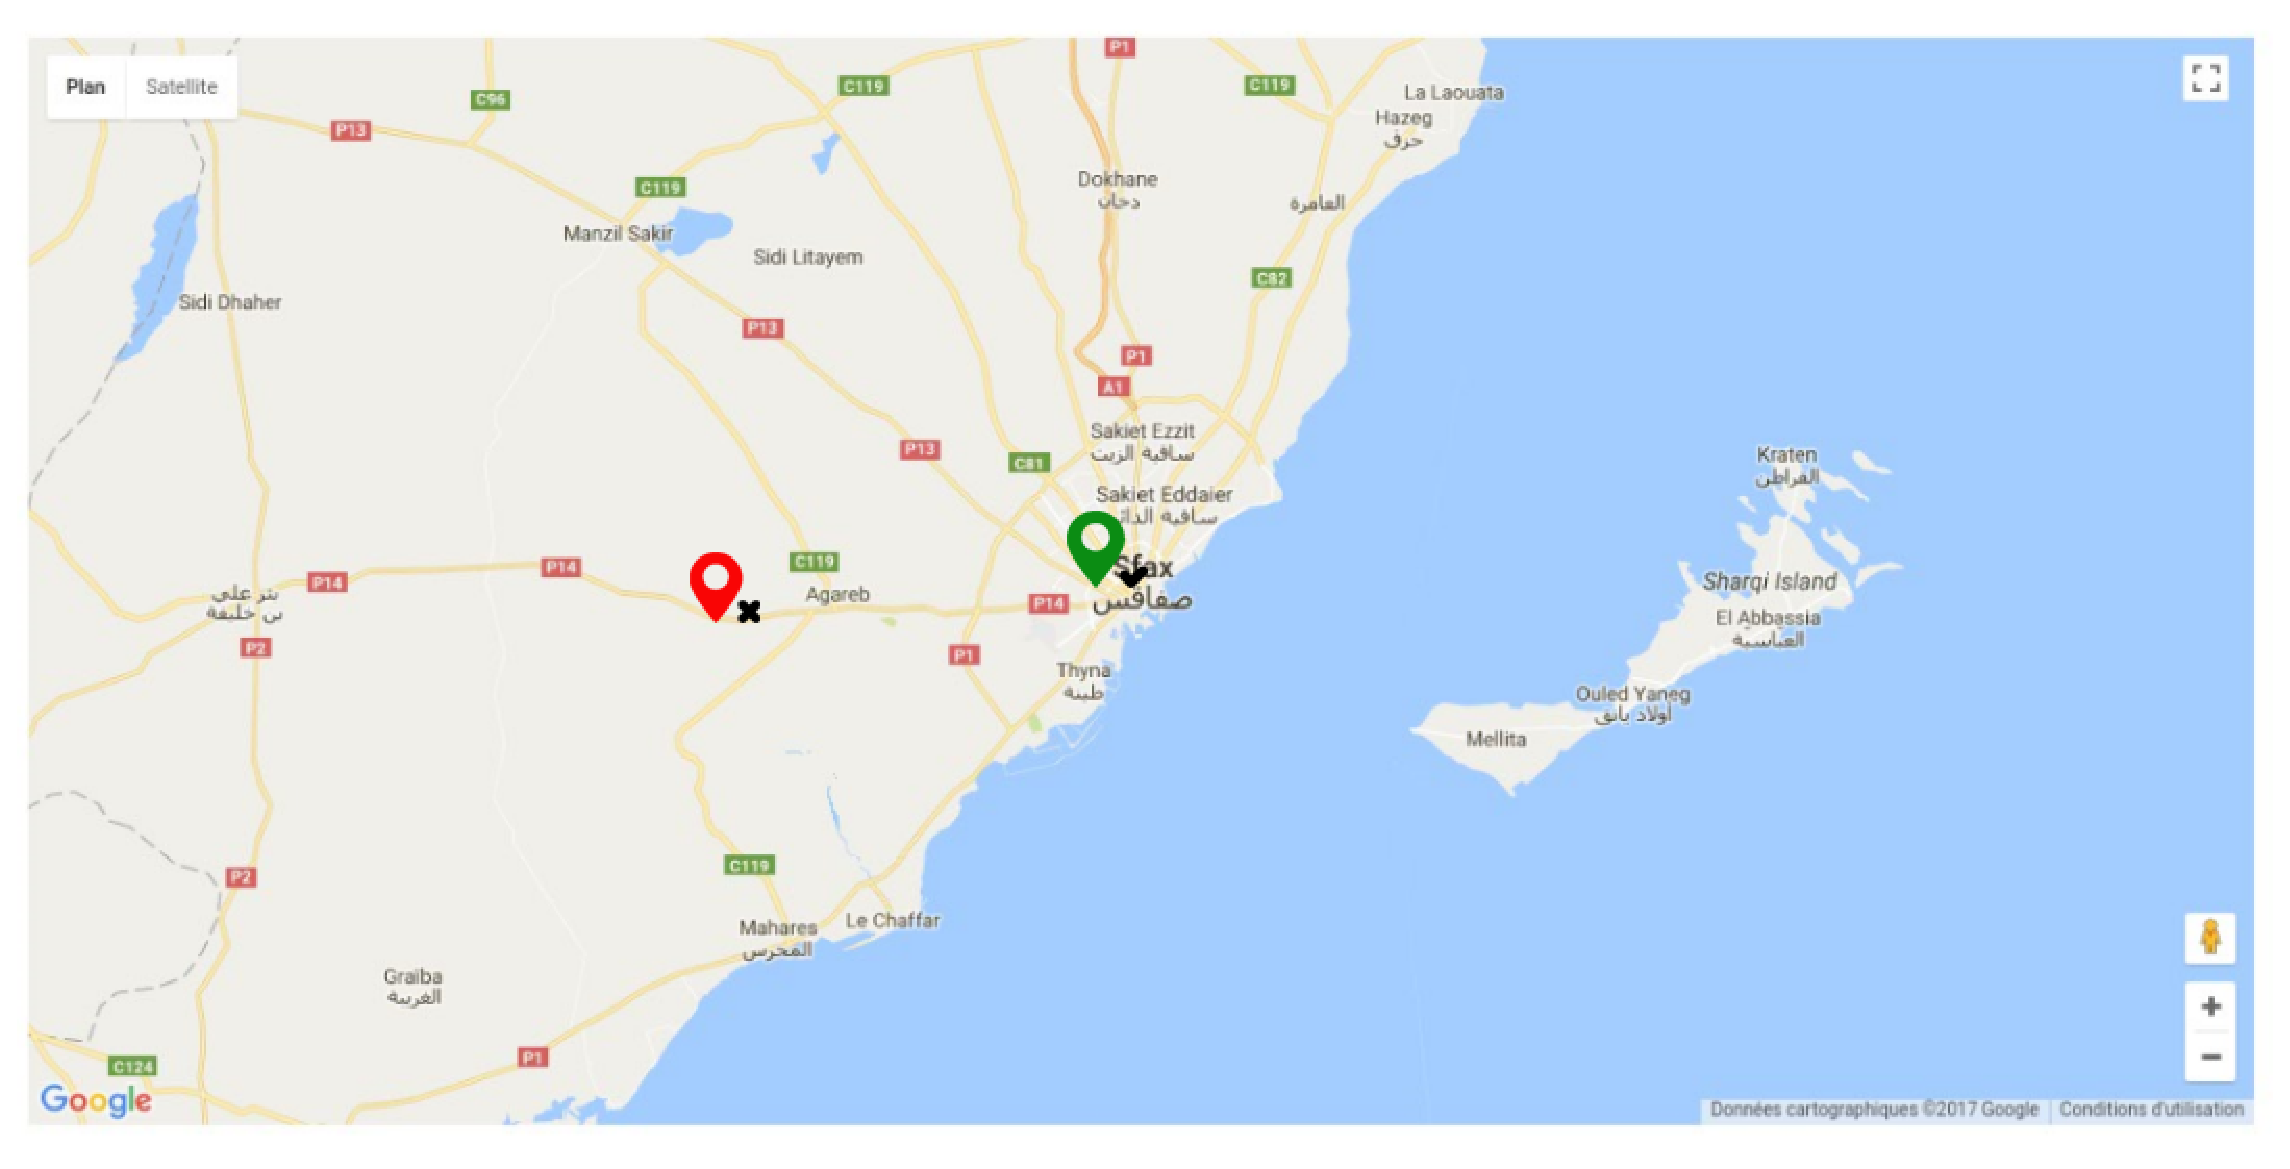
\includegraphics[width=0.6\textwidth]{sprint1-dashboard-screenshot}
    \caption{Capture écran de la page web de l'itération 1}
    \label{fig:sprint1-dashboard-screenshot}
\end{figure}

\paragraph{Application Android}

La figure~\ref{fig:sprint1-android-screenshot} représente l'interface de
l'application.

\begin{figure}[htbp]
    \centering
    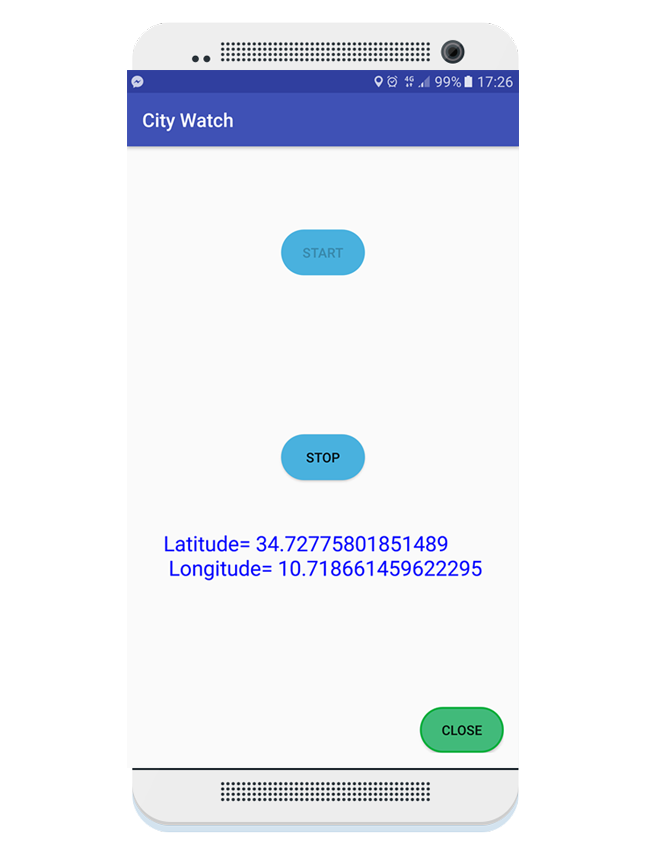
\includegraphics[width=0.45\textwidth]{sprint1-android-screenshot}
    \caption{Capture écran d'application Android de l'itération 1}
    \label{fig:sprint1-android-screenshot}
\end{figure}

\subsubsection{Avis du Product Owner}

Le Product Owner était ravi des résultats de cette première itération. Il a
validé donc notre travail et nous a encouragé pour l'élaboration des suivantes
itérations.

\subsubsection{Burndown chart}

La figure~\ref{fig:sprint1-burndown} présente une vue d'ensemble sur le progrès
de notre travail au cours de l'itération par rapport au progrès idéal.

\usetikzlibrary{plotmarks}

\begin{figure}
\centering
\begin{tikzpicture}[y=.2cm, x=.7cm,font=\sffamily]
\begin{axis}[
xlabel=$Jours$,
ylabel=$Heures\ restantes$,
grid=both,
grid style={line width=.1pt, draw=gray!10},
width=0.8\textwidth,
height=6cm,
%major grid style={line width=.2pt,draw=gray!50},
]
\addplot[color=blue,mark=*] coordinates {
        (0,30)
        (7, 0)
    };
    \addlegendentry{Temps Idéal}

    \addplot[mark=*,red] plot coordinates {
        (0, 30)
        (1, 25)
        (2, 20)
        (3, 12)
        (4, 8)
        (5, 4)
        (6, 0)
        (7, 0)
    };
    \addlegendentry{Temps Restant}
\end{axis}
\end{tikzpicture}
\caption{Graphique d'avancement - Itération 1}
\end{figure}


\subsection{Conclusion}
A la fin de cette itération, on avait un prototype minimale fonctionnel
dont on peut baser notre future travail.
L'approche suivi de faire le minimum des taches pendant la première itération
avait des bon effet sur les membre de notre équipe sur tout la motivation et
la solidarité.

Le tableau~\ref{tab:sprint1-evaluation} présente le pourcentage de
réalisation de nos taches de cette itération.

\begin{center}
    \begin{longtable}{| l | l |}
        \caption{Liste des tâches réalisées de la première itération}
        \label{tab:sprint1-evaluation} \\

        \hline
        \textbf{Les tâches} & \textbf{Taux de réalisation} \\ \hline
        \endhead

        \hline \multicolumn{2}{|r|}{{Continué en page suivante$\dotsc$}} \\ \hline
        \endfoot

        \hline \hline
        \endlastfoot

        \hline
Présentation et Configuration SVN & Effectué 100\% \\ \hline
Recherche sur les Services Web & Effectué 100\% \\ \hline
Implémenter service Save Position & Effectué 100\% \\ \hline
Implémenter la consommation du service Save Position & Effectué 100\% \\ \hline
Recherche sur les spécifications de la plateforme Android & Effectué 100\% \\ \hline
Création squelette de l'application mobile & Effectué 100\% \\ \hline
Implémenter service Get Last Position & Effectué 100\% \\ \hline
Rectification service Save Positon & Effectué 100\% \\ \hline
Rectification service Get Last Position & Effectué 100\% \\ \hline
Affiche Multiple marqueurs & Effectué 100\% \\ \hline
Affiche état du périphérique & Effectué 100\% \\ \hline
    \end{longtable}
\end{center}

\section[Itération 2: ( 3/8/2017 - 3/28/2017 )]{Itération~2:~\textup{\textto{(~3/8/2017~-~3/28/2017~)}}}

\subsection{Introduction}

\subsection{L'objectif du sprint}

L'objectif de cette itération vise trois environnements. Nous allons ajouter
une nouvelle vision par rapport à l'itération précédentes.

Ils sont comme suit:

\begin{description}
    \item [Smartphone] L'ajout de nouvelles fonctionnalités comme:
        \begin{itemize}
            \item La capture de l'embouteillage.
            \item La détection des secousses.
            \item La déclaration des ralentisseurs.
        \end{itemize}
    \item [Dashboard] Enrichir la carte par:
        \begin{itemize}
            \item Des nouveaux marqueurs qui spécifient chaque type de rapport
                ajouté.
            \item Une légende pour le filtrage des marqueurs.
        \end{itemize}
    \item [Rapport] La création d'une page rapport qui permet à l'utilisateur
        de:
        \begin{itemize}
            \item Faire une description sur le type du rapport(violence,
                accident, déchet, \ldots)
            \item Charger une image.
            \item Choisir sa position automatiquement ou manuellement.
        \end{itemize}
\end{description}

%La méthodologie Scrum a eu un impact positif sur les développeurs, du point de
%vue social, elle a valorisé le travail en équipe, la solidarité, le respect et
%la communication entre toutes les parties prenantes (client, développeurs,
%\ldots). Elle a aussi changé leur vison sur le développement des logiciels.

%L'objectif de cette itération est d'ajouter un système de gestion des rapport,
%d'améliorer la qualité de service web de location et d'enrichir des
%fonctionnalités du \textquote{Dashboard}.

\subsection{Planification de l'itération 2}

Au sein de la réunion de planification nous avons sélectionné les tâches à
réaliser au cours de cette itération tout en accord avec le \textquote{Product
Owner}.

\subsubsection{Backlog de l'itération}

\begin{center}
    \footnotesize
    \begin{longtable}{| p{1cm} | p{5cm} | p{7cm} | p{1cm} |}
        \caption{backlog de l'itération 2}
        \label{tab:sprint2-backlog} \\

        \hline
        \multicolumn{1}{|c}{\textbf{Réf}} &
        \multicolumn{1}{|c}{\textbf{Spécification}} &
        \multicolumn{1}{|c}{\textbf{Description}} &
        \multicolumn{1}{|c|}{\textbf{Priorité}} \\ \hline
        \endhead

        \hline \multicolumn{4}{|r|}{{Continué en page suivante$\dotsc$}} \\ \hline
        \endfoot

        \hline \hline
        \endlastfoot

        \hline
1 & Recherche sur les trajectoires & Comment présenter et enregistrer les trajectoire & 1 \\ \hline
2 & Affichage du trajet sur la carte & Visualizer le trajectoire d'un périphérique comme un ligne & 1 \\ \hline
3 & Implementer service d'enregsitrement des ralentisseurs & Enregistrer les données nécessaires pour représenter un ralentisseur & 1 \\ \hline
4 & Responsive design & IHM de l'applicaiont Android adaptable aux differents résolutions et rotations & 2 \\ \hline
5 & Implementer l'interface de déclaration un ralentisseur & Boutton rapport activé seulement si la localisation est active & 2 \\ \hline
6 & Filtrage des marqueurs dans la carte & Légende simplifiée permettant de choisir les types de données affichés dans la carte & 1 \\ \hline
7 & Implementer service de chargement de l'image & Charger, valider et enregistrer les images dans le serveur & 1 \\ \hline
8 & Implementer la fonctionnalité de déclaration des rapports & Formulaire avec validation et service d'enregistrement dans le serveur & 1 \\ \hline
9 & Recherche test unitaires & Comment améliorer la qualité du code et installation d'une solution des tests unitaires & 1 \\ \hline
10 & Recherche sur les frameworks PHP & Choisir le framework optimal pour notre platform et faire la migration & 2 \\ \hline
11 & Groupement de secousse sur la carte & Les marquers de secousses regroupés lors d'un zoom out sur la carte et séparer lors d'un zoom in & 3 \\ \hline
    \end{longtable}
\end{center}

\subsubsection{Estimation de la deuxième itération}

Comme l'itération précédant, Nous avons fixé la période de cette itération à 3
semaine.

\begin{table}[htbp]
    \centering
    \begin{tabular}{| c | c | c | c |}
        \hline
        \textbf{Membre} & \textbf{Nombre d'heures par jour} & \textbf{Nombre de jours présent} & \textbf{Total en heures} \\ \hline
        \hline
Moez & 8 & 18& 144\\ \hline
Rihab & 8 & 18 & 144 \\ \hline
\multicolumn{2}{c|}{} & \textbf{Total} & 288 \\ \cline{3-4}
    \end{tabular}
    \caption{Nombre d'heures de travail estimé de l'itération 2}
    \label{tab:sprint2-capacity}
\end{table}

\begin{center}
    \begin{longtable}{| l | l | l |}
        \caption{Nombre d'heures estimé pour la réalisation des taches}
        \label{tab:sprint2-estimation} \\

        \hline
        \multicolumn{1}{|c}{\textbf{Spécification}} &
        \multicolumn{1}{|c}{\textbf{Membre}} &
        \multicolumn{1}{|c|}{\textbf{Heures}} \\ \hline
        \endhead

        \hline \multicolumn{3}{|r|}{{Continué en page suivante$\dotsc$}} \\ \hline
        \endfoot

        \hline \hline
        \endlastfoot

        \hline
Recherche sur les trajectoires & Rihab & 5 x 2 \\ \hline
Affichage du trajet sur la carte & Moez & 13 x 2 \\ \hline
Implementer service d’enregsitrement des ralentisseurs & Moez & 5 \\ \hline
Responsive design & Rihab & 5 x 2 \\ \hline
Implementer l’interface de déclaration d'un ralentisseur & Rihab & 13 x 2 \\ \hline
Filtrage des marqueurs dans la carte & Rihab & 13 \\ \hline
Implementer service de chargement de l'image & Moez & 5 \\ \hline
Implementer la fonctionnalité de déclaration des rapports & Moez & 5 \\ \hline
Recherche test unitaires & Moez & 5 \\ \hline
Recherche sur les frameworks PHP & Moez & 5 \\ \hline
Groupement de secousse sur la carte & Rihab & 5 \\ \hline
    \end{longtable}
\end{center}

%\subsubsection{Évolution du travail}

\subsection{Présentation des outils utilisés}

\subsubsection{Lumen}

On a décidé de migrer vers un framework pour le développement du backend du
notre plateforme dans le but de simplifier et améliorer nos services web. Les
critères de choisir le framework étaient sa performance, sa stabilité et son
support de développement des api RESTful. Les 3 frameworks principales étudiés:

\begin{description}
    \item [Slim] Un macro framework performant avec support de développement
        des services web de premiere classe. Il manque le support pour
        développer des sites web classiques.
    \item [Symfony] Le framework PHP de référence. Il suivre une architecture
        modulaire et fournit une haute performance. Pour ajouter le support des
        services web, il nécessite l'ajoute et configurations des multiples des
        extensions.
    \item [Lumen] Une version minimal du framework Laravel pour le
        développement des services web. Étant basé sur Laravel, il profile d'un
        excellent support des extensions du troisième partie.
\end{description}

Lumen était choisi pour sa simplicité de configurer et de lancer et pour son
support de migrer vers Laravel en cas ou on aura besoin de supporter le
développement du site web classique ou autres types de développement.


%Pour le développement de backend du notre plateforme, la langue du
%programmation PHP a été pré choisi. Mais, on avait la responsabilité de choisir
%les bibliothèques et les frameworks. Pendant la 1\iere{} itération, le but
%était de se familiariser avec la langue PHP\@. Donc, on a utilisé seulement les
%extensions officiel du PHP incluant PDO, \ldots. Dans l'itération suivante, on
%a étudié les frameworks disponibles. A la fin, on a choisi le framework Lumen
%qui est une version simplifié du Laravel pour le développement des API
%\acrshort{RESTful}.

\subsection{Mises des normes}

Outres que les critères de la premiere itération, les nouveaux critères à
respecter pour cette itération sont:

\paragraph{Qualité du trajectoire}
Le trajectoire doit être aligné sur le trajet avec bonne précision. Et le
nombre des positions nécessaire pour tracer le trajectoire doivent être le
minimum le plus possible.

\paragraph{Architecture modulaire}
Architecture de backend doit être modulaire: On doit changer notre code
procédurale par un code orienté objet et minimiser la duplication du code et
séparer le code des models et le code des contrôleurs.

\paragraph{IHM de la page Dashboard Responsive}
Affiche claire et responsive des marqueurs dans la carte meme si le nombre est
très élevé.

\subsection{Modélisation UML}

\begin{figure}[htbp]
    \centering
    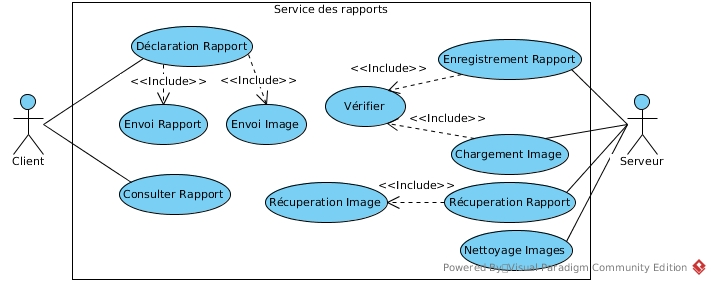
\includegraphics[width=1\textwidth]{sprint2-webservices-report-usecase}
    \caption{Diagramme de case d'utilisation du services Rapports en itération 2}
\end{figure}

\begin{figure}[htbp]
    \centering
    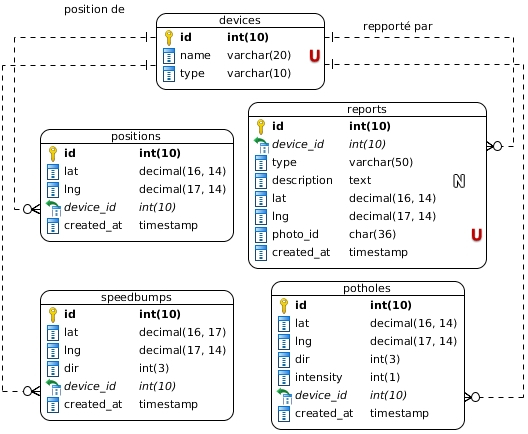
\includegraphics[width=1\textwidth]{sprint2-webservices-database}
    \caption{Diagramme entité-association du service Position en itération 2}
\end{figure}

\begin{figure}[htbp]
    \centering
    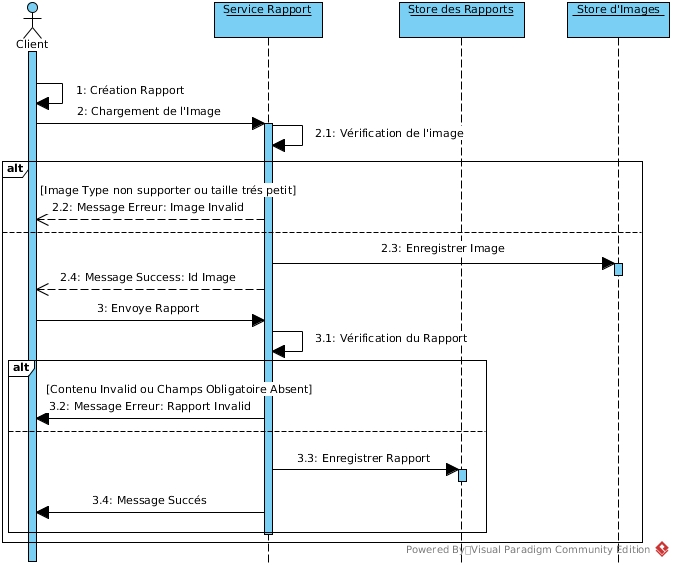
\includegraphics[width=1\textwidth]{sprint2-webservices-report-post-sequence}
    \caption{Diagramme de séquence du services Post Rapports en itération 2}
\end{figure}

\begin{figure}[htbp]
    \centering
    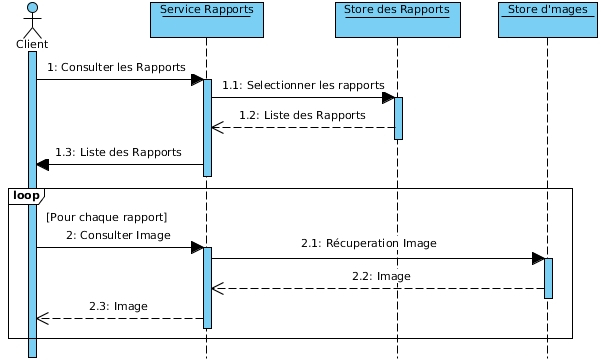
\includegraphics[width=1\textwidth]{sprint2-webservices-report-get-sequence}
    \caption{Diagramme de séquence du services Get Rapports en itération 2}
\end{figure}

\begin{figure}[htbp]
    \centering
    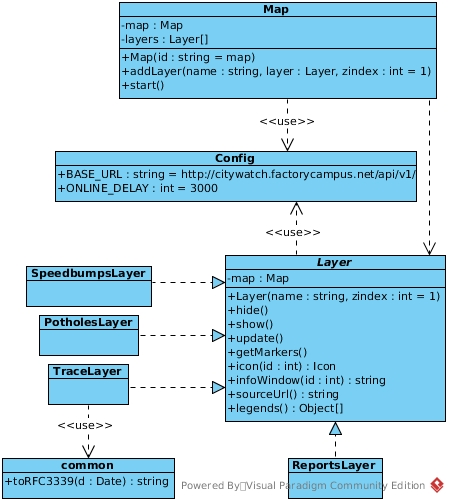
\includegraphics[width=0.9\textwidth]{sprint2-dashboard-class}
    \caption{Diagramme des classes du Dashboard}
    \label{fig:sprint2-dashboard-class}
\end{figure}

\subsection{Évaluation suivant les normes mise}

\TODO{EVALUATION}

\subsection{Contributions}

Au cours de l'itération avec l'augment des fonctionnalités ajoutées au
Dashboard, le code JavaScript devenu complexe, dupliqué et difficile à détecter
les bugs. On a décidé de réécrire le code avec une architecture modulaire et
plus moderne.

L'utilisation de la version ECMAScript 6 du JavaScript nous a fourni les
techniques de base nécessaires comme POO, Template Strings, paramètres par
défaut, nouvelles variantes de la boucle For et support de la programmation
asynchrone.

La nouvelle architecture est décrite dans le
diagram~\ref{fig:sprint2-dashboard-class}. Elle consiste de:

\begin{itemize}
    \item Une classe \verb|Map| contenu tout le logique métier d'initialiser et
        afficher la carte, registre et filtrer des différents types de données
        et traiter les différents évènements d'interaction humaine machine.
    \item Une classe abstract \verb|Layer| contenu tout le logique relié à
        chaque types des données à visualiser dans la map (téléchargement
        continuellement les données, génération les marqueurs ou zones, mise à
        jour des données, définition des filtrages supportés et les
        informations additionnelles à afficher). Le code commun entre
        différents layers est implémenté dans cette classe abstract.
    \item Une classe pour chaque type de données à visualiser (trajectoire,
        ralentisseurs, secousses, \ldots) qui hérite du classe \verb|Layer|. La
        plupart du temps, on a juste besoin de définir l'URL du resource, la
        listes des icons et des filtrages possibles.
    \item Un espace de noms \verb|Config| contenu les variables de
        configuration.
\end{itemize}

\subsection{Revue de cette itération}

\subsubsection{Produit de l'itération}

A la fin de l'itération 2, nous détaillons les différentes spécifications qui
caractérisent et implémenté le système de gestion des rapport.

\paragraph{Page \textquote{Rapport}}

Dans cette page, nous donne la main à l'utilisateur pour faire un petit rapport
comme expliqué dans la figure~\ref{fig:sprint2-rapport-screenshot1}. Cette page
permet à l'utilisateur d'envoyer son rapport au serveur pour l'enregistrer. La
position du rapport est détecté automatique à travers l'api JavaScript standard
Location. On donne la main à l'utilisateur pour changer la location
manuellement en glissant le marqueur ou en changer les inputs. Le chargement de
l'image est obligatoire.

\TODO{Cette obligation était éliminer en review}

L'envoie du rapport est éxecuté en deux phases:

\begin{enumerate}
    \item Chargement de l'image au serveur. Si le type et le taille de l'image
        est valide, le serveur retourne un id unique (UUID) de l'image.
    \item Envoie du rapport au serveur. Les informations envoyées sont: type du
        rapport, id image, commentaire (optionnel) et les coordonnées.
\end{enumerate}

\begin{figure}[htbp]
    \centering
    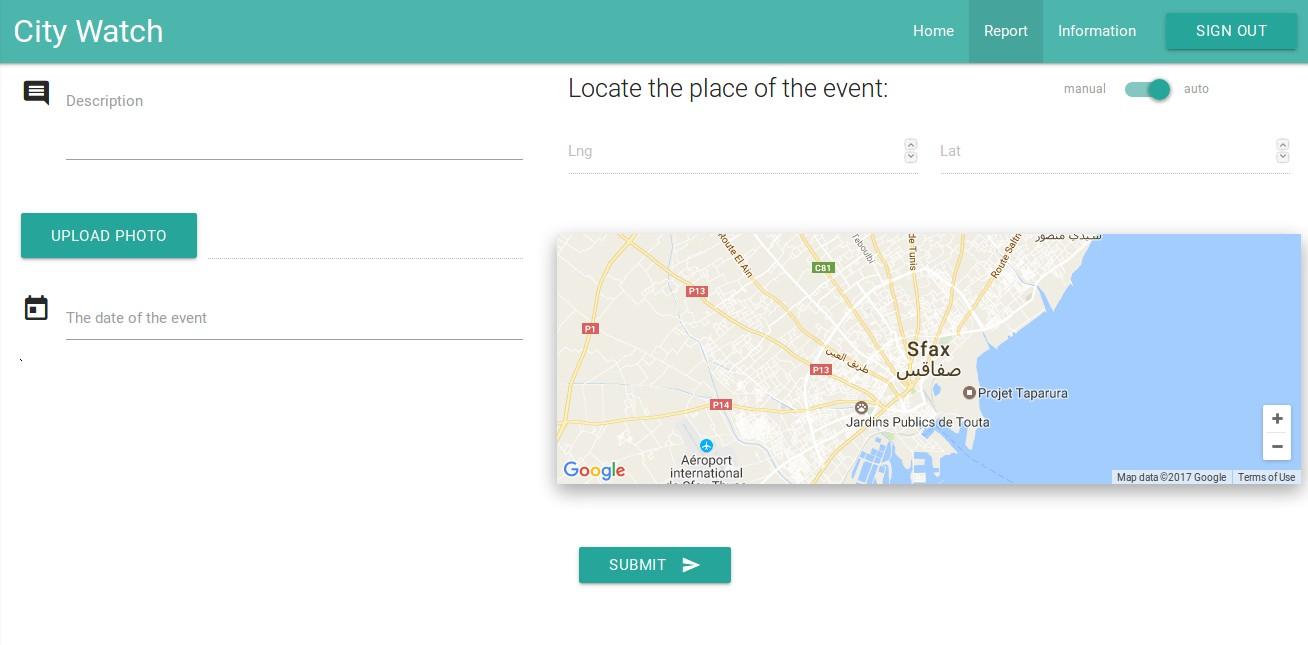
\includegraphics[width=0.7\textwidth]{sprint2-rapport-screenshot1}
    \caption{Page Rapport}
    \label{fig:sprint2-rapport-screenshot1}
\end{figure}

\paragraph{Page \textquote{Dashboard}}
L'utilitaire de regroupement de marqueurs vous aide à gérer plusieurs marqueurs
à différents niveaux de zoom. Précisément, les marqueurs sont en fait des
éléments à ce stade et ne deviennent réellement des marqueurs qu'après leur
rendu. Par souci de clarté, nous ne parlerons que de marqueurs dans ce
document.

Lorsqu'un utilisateur affiche la carte à un niveau de zoom élevé comme montre
la figure~\ref{fig:sprint2-dashboard-screenshot1}, les différents marqueurs
s'affichent sur la carte. Lorsqu'il effectue un zoom arrière comme montre la
figure~\ref{fig:sprint2-dashboard-screenshot2}, les marqueurs se regroupent
pour faciliter la consultation de la carte.

\begin{figure}[htbp]
    \begin{subfigure}{.5\textwidth}
        \centering
        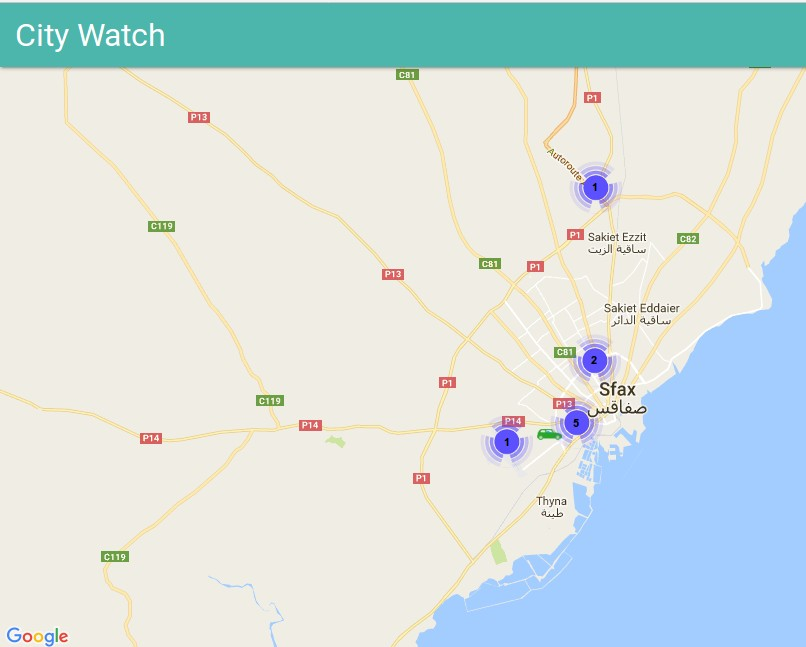
\includegraphics[width=.8\linewidth]{sprint2-dashboard-screenshot1}
        \caption{Groupement activé en un zoom bas}
        \label{fig:sprint2-dashboard-screenshot1}
    \end{subfigure}
    \begin{subfigure}{.5\textwidth}
        \centering
        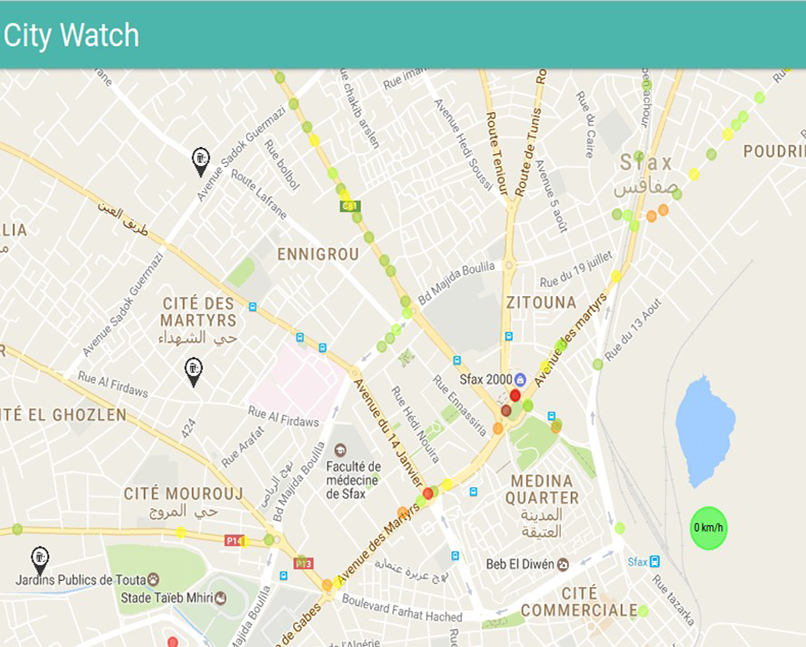
\includegraphics[width=.93\linewidth]{sprint2-dashboard-screenshot2}
        \caption{Groupement désactivé en zoom haut}
        \label{fig:sprint2-dashboard-screenshot2}
    \end{subfigure}
    \caption{Groupement des marqueurs des secousses en différents niveaux du zoom}
\end{figure}

\paragraph{Application Mobile \textquote{CityWatch}}

Dans notre application, l'utilisateur doit s'inscrit pour accéder à
l'application. Les données saisies dans le formulaire d'inscription (nom
d'utilisation, mot de passe) seront envoyées et stockées en toute sécurité et
confidentialité. Lorsqu'un utilisateur tend à se connecter, il tape son mot de
passe déjà saisies dans le formulaire d'inscription, alors une vérification
avec le serveur doit avoir lieu.

\textbf{Note:} Pour chaque nom d'utilisateur ajouté, le serveur vérifie
l'unicité de ce dernier.

\begin{figure}[htbp]
    \begin{subfigure}{.5\textwidth}
        \centering
        \centering
        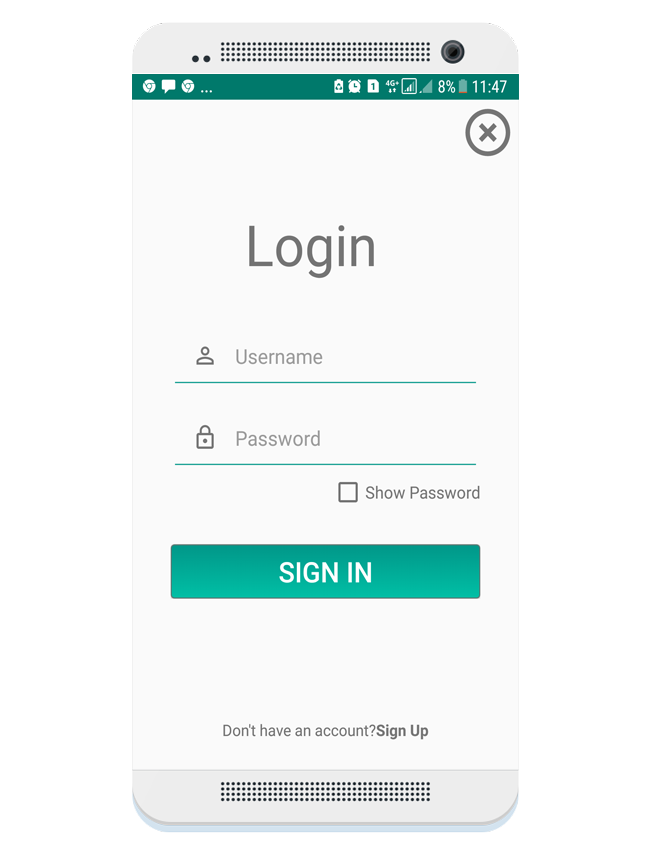
\includegraphics[width=.7\linewidth]{sprint2-android-screenshot1}
        \caption{Activité du confection}
        \label{fig:sprint2-android-screenshot1}
    \end{subfigure}
    \begin{subfigure}{.5\textwidth}
        \centering
        \centering
        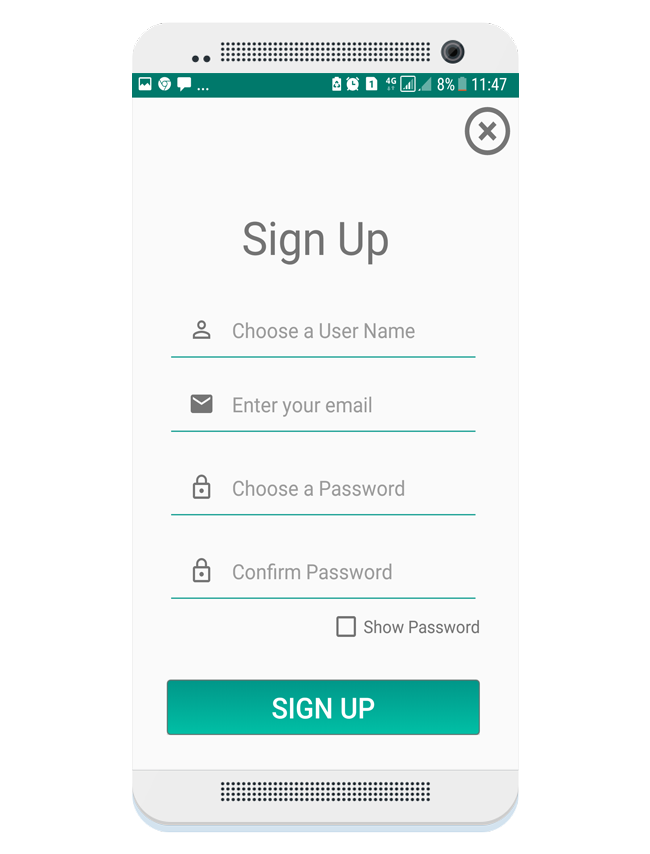
\includegraphics[width=.7\linewidth]{sprint2-android-screenshot2}
        \caption{Activité d'inscription}
        \label{fig:sprint2-android-screenshot2}
    \end{subfigure}
    \caption{Formulaire d'inscription}
\end{figure}

\subsubsection{Avis du Product Owner}

A la fin de cette première itération, nous avons présenté au \textquote{Product
Owner} le produit obtenu. Le \textquote{Product Owner} a exprimé sa
satisfaction du travail.

\subsubsection{Graphique d'avancement de l'itération}

\usetikzlibrary{plotmarks}

\begin{figure}
\centering
\begin{tikzpicture}[y=.1cm, x=.7cm,font=\sffamily]
\begin{axis}[
xlabel=$Jours$,
ylabel=$Heures\ restantes$,
grid=both,
grid style={line width=.1pt, draw=gray!10},
width=0.9\textwidth,
height=10cm,
%major grid style={line width=.2pt,draw=gray!50},
]
\addplot[color=black,mark=*] coordinates {
        (0,144)
        (18,0)
    };
    \addlegendentry{Temps Idéal}

    \addplot[mark=*,red] plot coordinates {
        (0, 144)
        (1, 138)
        (2, 130)
        (3, 125)
        (4, 122)
        (5, 115)
        (6, 111)
        (7, 108)
        (8, 100)
        (9, 92)
        (10, 88)
        (11, 88)
        (12, 85)
        (13, 80)
        (14, 72)
        (15, 60)
        (16, 55)
        (17, 48)
        (18, 40)
       
    };
    \addlegendentry{Rihab}
      \addplot[mark=*,cyan] plot coordinates {
        (0, 144)
        (1, 130)
        (2, 125)
        (3, 120)
        (4, 110)
        (5, 100)
        (6, 100)
        (7, 100)
        (8, 98)
        (9, 90)
        (10, 82)
        (11, 73)
        (12, 72)
        (13, 60)
        (14, 49)
        (15, 41)
        (16, 35)
        (17, 30)
        (18, 22)
       
    };
    \addlegendentry{Moez}
\end{axis}
\end{tikzpicture}
\caption{Graphique d'avancement - Itération 2}
\end{figure}

\subsection{Conclusion}
\begin{center}
    \begin{longtable}{| l | l |}
        \caption{Liste des tâches réalisées de deuxième itération }
        \label{tab:sprint2-estimation} \\

        \hline
        \textbf{Les tâches} & \textbf{Taux de réalisation} \\ \hline
        \endhead

        \hline \multicolumn{2}{|r|}{{Continué en page suivante$\dotsc$}} \\ \hline
        \endfoot

        \hline \hline
        \endlastfoot

        \hline
Recherche sur les trajectoires & Effectué 100\% \\ \hline
Affichage du trajet sur la carte & Effectué 100\% \\ \hline
Implementer service d’enregsitrement des ralentisseurs & Effectué 100\% \\ \hline
Responsive design & Effectué 80\% \\ \hline
Implementer l’interface de déclaration d'un ralentisseur & Effectué 100\% \\ \hline
Filtrage des marqueurs dans la carte & Effectué 100\% \\ \hline
Implementer service de chargement de l'image & Effectué 80\% \\ \hline
Implementer la fonctionnalité de déclaration des rapports & Effectué 100\% \\ \hline
Recherche test unitaires & Effectué 80\% \\ \hline
Recherche sur les frameworks PHP & Effectué 100\% \\ \hline
Groupement de secousse sur la carte & Effectué 100\% \\ \hline
    \end{longtable}
\end{center}

\backgroundsetup{contents=WIP,scale=8,position={0.9,-1.5},opacity=0.6}
\section[Itération~3:~(~4/3/2017~-~4/28/2017~)]{Itération~3:~\textup{\textto{(~4/3/2017~-~4/28/2017~)}}}

\subsection{Introduction}

\subsection{L'objectif du sprint}

En accord avec le product owner,le but de cette itération est:

\begin{description}
    \item [Smartphone] L’ajout de nouvelles fonctionnalités comme:
        \begin{itemize}
            \item La détection des réseaux avec leur intensité.
            \item l'exploitation des donnes collecté selon le besoin.
        \end{itemize}
    \item [Rapport] Typage des rapports.
    \item [Dashboard]
        \begin{itemize}
            \item Élaboration des mécanisme d'authentification.
            \item Des nouveaux marqueurs qui spécifient chaque type de rapport
                ajouté.
        \end{itemize}
\end{description}

%Le Product Owner nous a demandé d’améliorer le chargement de l'image
%dans le serveur de telle sorte que la qualité d'image reste la même..
%Donc, dans cette itération, nous allons tenir compte des attentes du Product Owner. Nous allons
%modifier le critère de chargement, En plus nous allons implémenter une méthode
%permettant de maintenir la qualité.

\subsection{Planification de l'itération 3}

\subsubsection{Backlog de l'itération}

Le but de cette itération est d'ajouter un système de gestion des rapport et d'améliorer
la qualité.

\begin{center}
    \footnotesize
    \begin{longtable}{| p{1cm} | p{5cm} | p{7cm} | p{1cm} |}
        \caption{Taches à faire de la troisième itération}
        \label{tab:sprint3-backlog} \\

 \hline
 \multicolumn{1}{|c}{\textbf{Réf}} &
 \multicolumn{1}{|c}{\textbf{Spécification}} &
 \multicolumn{1}{|c}{\textbf{Description}} &
 \multicolumn{1}{|c|}{\textbf{Priorité}} \\ \hline
 \endhead

 \hline \multicolumn{4}{|r|}{{Continué en page suivante$\dotsc$}} \\ \hline
 \endfoot

 \hline \hline
 \endlastfoot

\hline
3.1 & Integration Dashboard et Rapport dans l'application android & Implémenté la méthode qui affiche les pages ``Dashboard et Rapport'' chacun a un bouton spécifié   & 1 \\ \hline
3.2 & Authentification Restful  & Ajouter l'authentification dans le serveur pour assurer la sécurité   & 1 \\ \hline
3.3 & landing page & créer une nouvel page Web  & 3\\ \hline
3.4 & Compte utilisateur & Base de données accecible depuis l'application et le web& 2 \\ \hline
3.5 & Post réseau & Methode POST Restful & 1 \\ \hline
3.6 & GET réseau & Methode GET Restful & 1 \\ \hline
3.7 & Post vitesse & Methode POST vitesse & 1 \\ \hline
3.8 & Get vitesse & Methode GET & 1 \\ \hline
3.9 & Appplication Android Responsive & Responsive design coter android & 3 \\ \hline
3.10 & IHM & l'ajout des boutons radio pour distinguer (pieton / voiture)(android) & 3 \\ \hline
3.11 & Recherche Business intelligence & BI & 2 \\ \hline
3.12 & Implantation des BD au BI & données accessible en BI & 2\\ \hline
3.13 & création Logo &Ajouter Logo dans l'application & 3 \\ \hline
3.14 & étude scénario commercial embouteillage & scénario de marketing& 2\\ \hline
3.15 & Rectification chargement image & \ldots & 1 \\ \hline
3.16 & étude scénario commercial secousses & scénario de marketing& 2\\ \hline
\end{longtable}
\end{center}

\subsubsection{Estimation de la deuxième itération}
\begin{table}[htbp]
    \centering
    \begin{tabular}{| c | c | c | c |}
\hline
\textbf{Membre} & \textbf{Nombre d'heures par jour} & \textbf{Nombre de jours présent} & \textbf{Total en heures} \\ \hline
\hline

Moez & 8 & 48 & 144\\ \hline
Rihab & 8 & 48 & 144 \\ \hline
\multicolumn{2}{c|}{} & \textbf{Total} & 288 \\ \cline{3-4}
    \end{tabular}
    \caption{Nombre d'heures de travail estimé de l'itération 3}
    \label{tab:sprint3-capacity}
\end{table}

\begin{center}
    \begin{longtable}{| l | l | l |}
        \caption{Nombre d'heures estimé pour la réalisation des taches}
        \label{tab:sprint3-estimation} \\

 \hline
 \multicolumn{1}{|c}{\textbf{Spécification}} &
 \multicolumn{1}{|c}{\textbf{Membre}} &
 \multicolumn{1}{|c|}{\textbf{Heures}} \\ \hline
 \endhead

 \hline \multicolumn{3}{|r|}{{Continué en page suivante$\dotsc$}} \\ \hline
 \endfoot

 \hline \hline
 \endlastfoot

\hline
Integration Dashboard et Rapport dans l'application android & Rihab & 5 x 2 \\ \hline
Authentification Restful& Rihab & 5 x 2 \\ \hline
landing page& Rihab & 5 x 2 \\ \hline
Compte utilisateur& Rihab & 5 x 2 \\ \hline
Post réseau& Rihab & 5 x 2 \\ \hline
GET réseau& Rihab & 5 x 2 \\ \hline
Post vitesse& Rihab & 5 x 2 \\ \hline
Get vitesse& Rihab & 5 x 2 \\ \hline
Appplication Android Responsive & Rihab & 5 x 2 \\ \hline
IHM & Rihab & 5 x 2 \\ \hline
Recherche Business intelligence& Rihab & 5 x 2 \\ \hline
Implantation des BD au BI& Rihab & 5 x 2 \\ \hline
création Logo& Rihab & 5 x 2 \\ \hline
Étude scénario commercial embouteillage& Rihab & 5 x 2 \\ \hline
Rectification chargement image & Rihab & 5 x 2 \\ \hline
Étude scénario commercial secousses & Rihab & 5 x 2 \\ \hline
\end{longtable}
\end{center}

\subsection{Présentation des outils utilisés}
\subsubsection{API REST}
Les API REST sont basées sur le protocole HTTP, qui signifie Hypertext Transfer Protocol.
C’est ce qui est au cœur du web! C’est un protocole qui définit la communication
entre les différentes parties du web. L’échange est basé sur des requêtes client et serveur.
Un client lance une requête HTTP, et le serveur renvoie une réponse.
Ce sont des méthodes qui définissent les requêtes que le client peut effectuer,
dont GET\footnote{Récupérer une ressource (ne modifie pas la ressource).}, PUT\footnote{Modifier une ressource.},
POST\footnote{Créer une ressource.}, DELETE\footnote{Supprimer une ressource.} encore plus.

\subsubsection{Business Intelligence}

la Business intelligence\footnote{Informatique décisionnelle} propose d'utiliser
les données transitant par le Système
d'information, données de production le plus souvent, en informations susceptibles
d'être exploitées à des fins décisionnelles.

Sur le plan pratique et technique, la Business Intelligence se compose d'une famille
d'outils informatiques et
de progiciels assurant le fonctionnement de la chaîne de traitement de l'information.

Les 4 fonctions de la chaîne décisionnelle comment s'explique la figure~\ref{fig:sprint3-businessintelligence} sont:
\begin{description}[align=right,labelwidth=1cm]
 \item [1] Collecter, nettoyer et consolider les données Extraire les données
 des systèmes de production et les adapter à un usage décisionnel.
 \item [2] Stocker Centraliser les données structurées et traitées afin qu'elles
 soient disponibles pour un usage décisionnel.
 \item [3] Distribuer Ou plutôt faciliter l'accessibilité des informations selon
 les fonctions et les types d'utilisation.
 \item [4] Exploiter ou comment assister du mieux possible l'utilisateur afin qu'il puisse extraire
 la substance de l'information des données stockées à cet usage.
\end{description}
\clearpage

\begin{figure}[htbp]
  \centering
  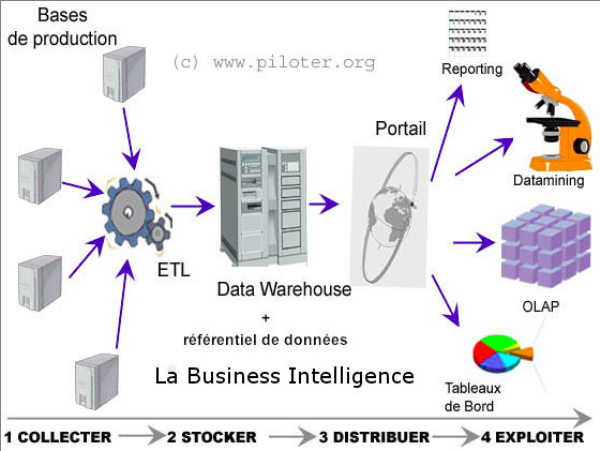
\includegraphics[width=0.8\textwidth]{sprint3-businessintelligence}
  \caption{Les 4 phases du processus de Business Intelligence}
  \label{fig:sprint3-businessintelligence}
\end{figure}


\subsection{Mises des normes}

\subsection{Modélisation UML}

\begin{figure}[htbp]
    \centering
    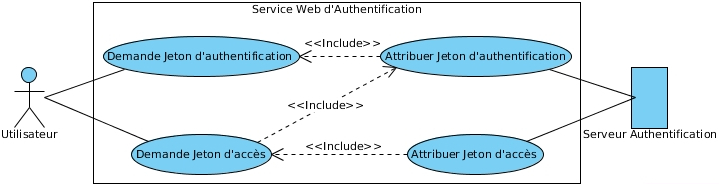
\includegraphics[width=1\textwidth]{sprint3-webservices-oauth-usecase}
    \caption{Diagramme de case d'utilisation du service d'Authentification en itération 3}
\end{figure}

\begin{figure}[htbp]
    \centering
    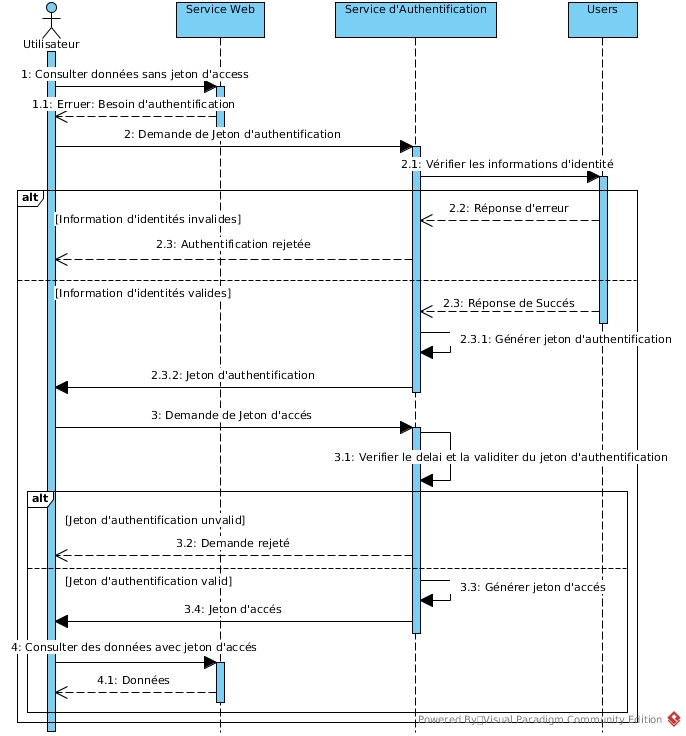
\includegraphics[width=1\textwidth]{sprint3-webservices-oauth-sequence}
    \caption{Diagramme de sequence du services d'Authentification en itération 3}
\end{figure}

\begin{figure}[htbp]
    \centering
    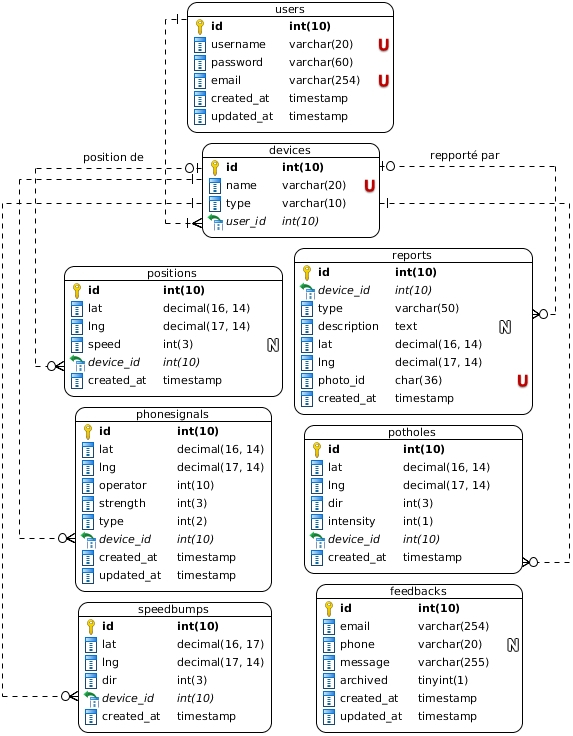
\includegraphics[width=1\textwidth]{sprint3-webservices-database}
    \caption{Diagramme d'entité-relation du services web en itération 3}
\end{figure}

\subsection{Évaluation suivant les normes mise}
\clearpage
\subsection{Revue de cette itération}
On rappelons que nous travaillons dans un équipe Scrum qui nécessite
l'intégration de notre travail dans le projet pour attentes le but.
\subsubsection{Produit de l'itération}
\paragraph{Légende du Dashboard}
Dans cette page nous travaillons alors sur deux parties:
\begin{itemize}
 \item la première : active/désactive les boutons de filtrage de chaque marqueur.
 \item la deuxième : gérés la communication interne entre serveur et la page.
 \end{itemize}
Aussi,nous participons 80\% à l'ajout de légende a notre carte
et affiche le filtrage des marqueurs.

\begin{figure}[htbp]
\centering
    \begin{subfigure}{.8\textwidth}
    \centering
  \centering
  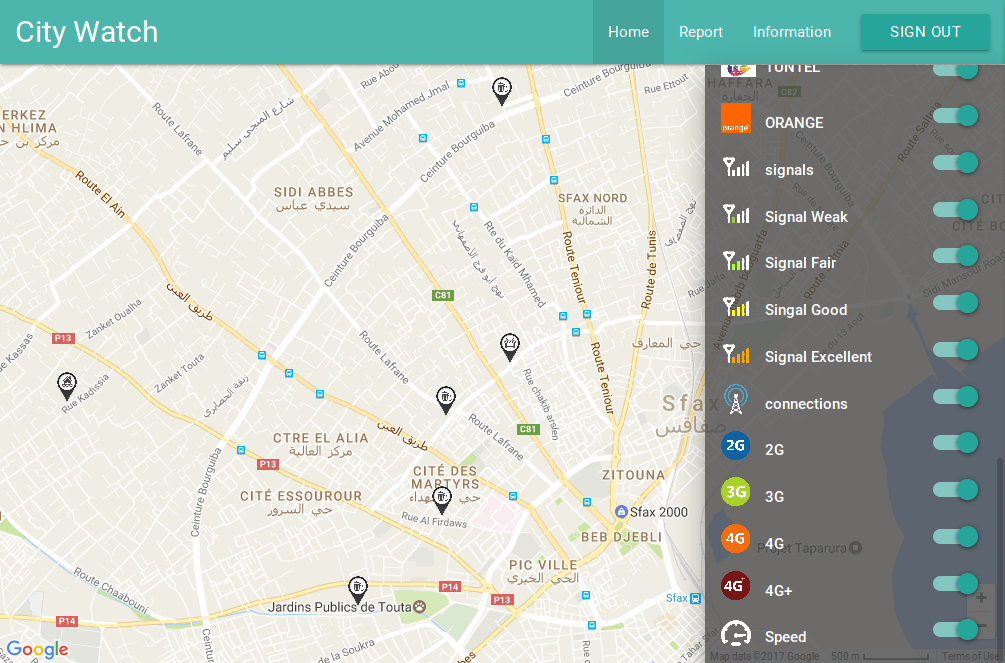
\includegraphics[width=1.0\linewidth]{sprint3-dashboard-screenshot1}
  \caption{Marqueurs activé}
  \label{fig:sprint3-dashboard-screenshot1}
\end{subfigure}
\begin{subfigure}{.8\textwidth}
    \centering
  \centering
  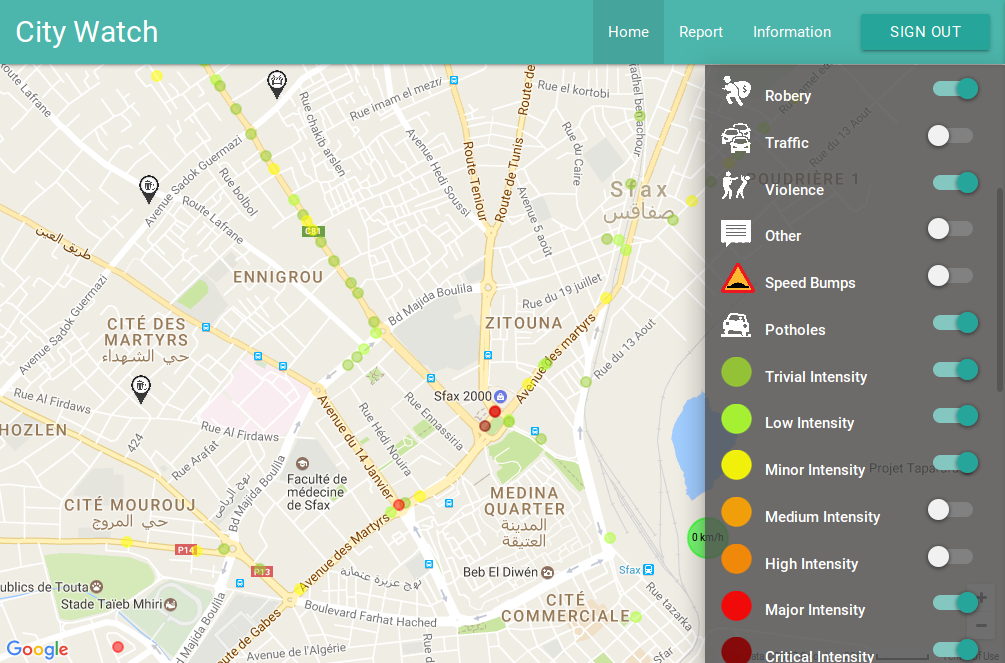
\includegraphics[width=1.0\linewidth]{sprint3-dashboard-screenshot2}
  \caption{Quelques marqueurs désactivé}
  \label{sprint3-dashboard-screenshot2}
\end{subfigure}
\caption{Dashboard CityWatch au troisième itération}
\end{figure}
\clearpage

\paragraph{Android}
\paragraph*{}
Les données captées par l'application mobile (Position , Secousses , Ralentisseur , Réseaux , force du 
signal et vitesse ) sont Récupérées par le serveur pour assurer la sauvegarde et la transmission vers une 
base données.\\

\begin{figure}[htbp]
\centering
    \begin{subfigure}{.45\textwidth}
    \centering
  \centering
  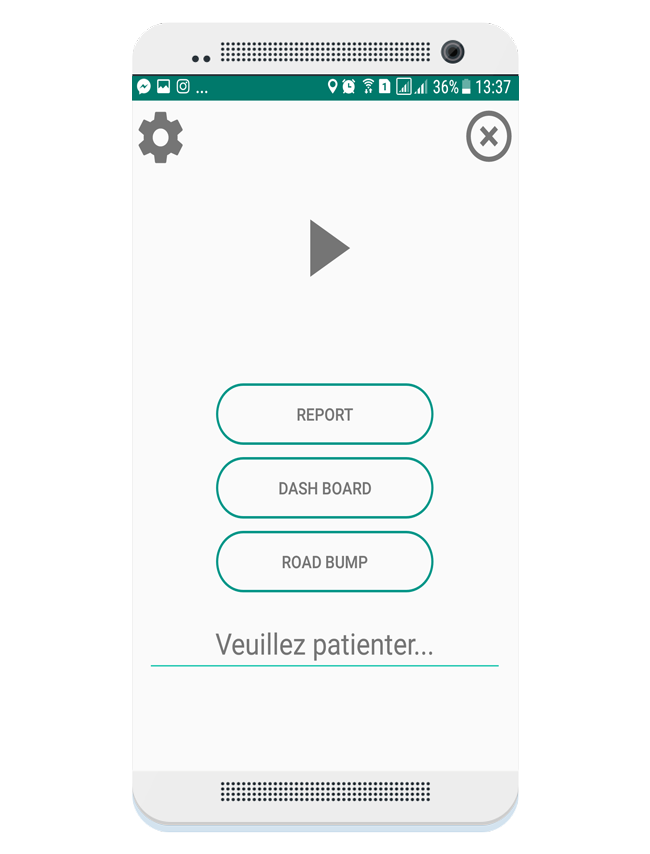
\includegraphics[width=1.0\linewidth]{sprint3-android-screenshot1}
  \caption{État désactivé}
  \label{fig:sprint3-android-screenshot1}
\end{subfigure}
\begin{subfigure}{.45\textwidth}
    \centering
  \centering
  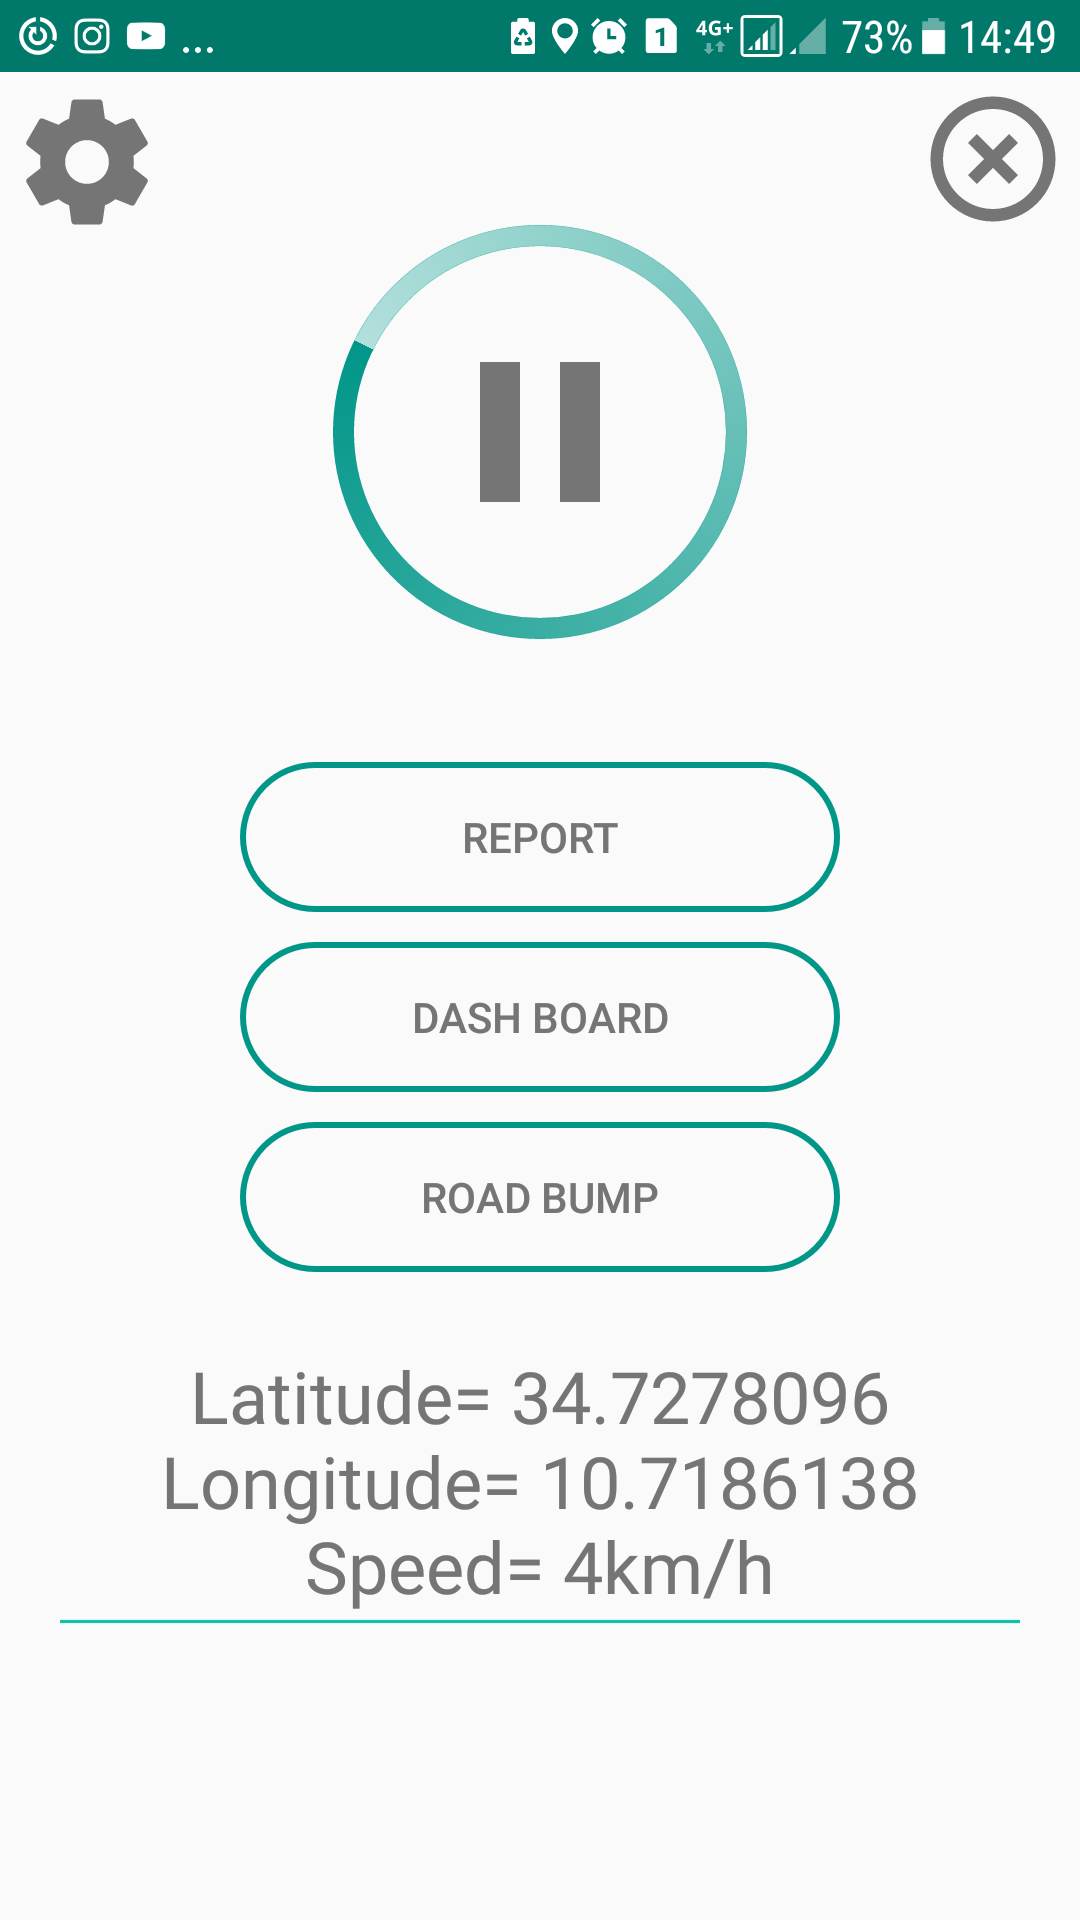
\includegraphics[width=1.0\linewidth]{sprint3-android-screenshot2}
  \caption{État activé}
  \label{fig:sprint3-android-screenshot2}
\end{subfigure}
\caption{Interface de l'application au troisième itération}
\end{figure}
\clearpage

\subsubsection{Avis du Product Owner}

Après la présentation du produit final, le \textquote{Product Owner} était très satisfait
a notre travail.

\subsubsection{Burndown chart}
La figure~\ref{fig:sprint3-burndown} présente une vue d'ensemble sur le progrès
de notre travail au cours de l'itération par rapport au progrès idéal.
\usetikzlibrary{plotmarks}

\begin{figure}
\centering
\begin{tikzpicture}[y=.2cm, x=.7cm,font=\sffamily]
\begin{axis}[
xlabel=$Jours$,
ylabel=$Heures\ restantes$,
grid=both,
grid style={line width=.1pt, draw=gray!10},
width=0.9\textwidth,
height=10cm,
%major grid style={line width=.2pt,draw=gray!50},
]
\addplot[color=black,mark=*] coordinates {
        (0,144)
        (18,0)
    };
    \addlegendentry{Temps Idéal}

    \addplot[mark=*,red] plot coordinates {
        (0, 144)
        (1, 138)
        (2, 130)
        (3, 122)
        (4, 111)
        (5, 104)
        (6, 95)
        (7, 85)
        (8, 55)
        (9, 55)
        (10, 42)
        (11, 33)
        (12, 33)
        (13, 33)
        (14, 21)
        (15, 15)
        (16, 13)
        (17, 2)
        (18, 0)
       
    };
    \addlegendentry{Rihab}
      \addplot[mark=*,cyan] plot coordinates {
       (0, 144)
        (1, 138)
        (2, 130)
        (3, 125)
        (4, 122)
        (5, 115)
        (6, 111)
        (7, 108)
        (8, 100)
        (9, 92)
        (10, 88)
        (11, 88)
        (12, 88)
        (13, 80)
        (14, 68)
        (15, 55)
        (16, 42)
        (17, 30)
        (18, 0)
       
    };
    \addlegendentry{Moez}
\end{axis}
\end{tikzpicture}
\caption{Graphique d'avancement - Itération 3}
\end{figure}

\subsection{Conclusion}

\begin{center}
    \begin{longtable}{| l | l |}
        \caption{Liste des tâches réalisées de la troisième itération}
        \label{tab:sprint3-estimation} \\

        \hline
        \textbf{Les tâches} & \textbf{Taux de réalisation} \\ \hline
        \endhead

        \hline \multicolumn{2}{|r|}{{Continué en page suivante$\dotsc$}} \\ \hline
        \endfoot

        \hline \hline
        \endlastfoot

        \hline
Integration Dashboard et Rapport dans l'application android & Effectué 100\% \\ \hline
Authentification Restful&  Effectué 100\% \\ \hline
landing page& Effectué 100\% \\ \hline
Compte utilisateur& Effectué 100\% \\ \hline
Post réseau& Effectué 100\% \\ \hline
GET réseau&  Effectué 100\% \\ \hline
Post vitesse&  Effectué 100\% \\ \hline
Get vitesse& Effectué 100\% \\ \hline
Appplication Android Responsive & Effectué 100\% \\ \hline
IHM & Effectué 100\% \\ \hline
Recherche Business intelligence& Effectué 100\% \\ \hline
Implantation des BD au BI & Effectué 30\% \\ \hline
création Logo&  Effectué 80\% \\ \hline
Étude scénario commercial embouteillage& Effectué 100\% \\ \hline
Rectification chargement image & Effectué 100\% \\ \hline
Étude scénario commercial secousses &  Effectué 100\% \\ \hline
\end{longtable}
\end{center}

\SetBgContents{}

%%%% INCLUDE CHAPTERS

\cleardoublepage
\renewcommand{\sectionmark}[1]{\markright{\thesection\ \ --\ \ #1}}
%\appendix
\begin{appendices}
\section{Annexe}
\pagebreak

\subsection{Documentation des Services Web d'itération 1}

\subsubsection{Service Post Position}
\label{appendix:sprint1-position-post-doc}

\textbf{POST} \ \texttt{/positions/\textit{:id}}

\begin{table}[htbp]
    \centering
    \caption*{Paramètres Service Post Position}
    \begin{tabular}{llll}
        \toprule
        \multicolumn{1}{c}{\textbf{Élément}} &
        \multicolumn{1}{c}{\textbf{Obligation}} &
        \multicolumn{1}{c}{\textbf{Type}} &
        \multicolumn{1}{c}{\textbf{Description}} \\
        \midrule
        \verb|:id| & obligatoire & string & identificateur du périphérique \\
        \verb|lat| & obligatoire & nombre [-90, 90] & latitude de la position \\
        \verb|lng| & obligatoire & nombre [-180, 180] & longitude de la position \\
        \verb|last_modified| & optionnel & string (RFC3339) & date du capture de la position \\
        \bottomrule
    \end{tabular}
\end{table}

\subparagraph*{Réponse Codes}
\begin{description}
    \item[\texttt{204 No Content}] Position était crée ou mette à jour avec succès.
    \item[\texttt{400 Bad Request}] Le contenu JSON n'est pas valide.
    \item[\texttt{422 Unprocessable Entity}] Entité obligatoire absente ou format d'une entité est invalide.
\end{description}

\subparagraph*{Entités de réponse}

n/a

\begin{listing}
    \caption*{Démonstration Service Post Position}
    \begin{minted}[label={Requéte}]{bash}
curl -i -X POST http://localhost/positions/1 \
     -d '{"lat": 10.71979600000000,
          "lat": "34.72563400000000",
          "last_modified": "2017-03-27 10:34:01"}' \
     -H 'Content-Type: application/json'
\end{minted}
\begin{minted}[label={Réponse en Succés}]{http}
HTTP/1.1 200 Success
Content-Type: application/json

{
    "success": true
}
\end{minted}
\end{listing}

\clearpage
\subsubsection{Service Get Position}
\label{appendix:sprint1-position-get-doc}

\textbf{GET} \ \texttt{/positions/\textit{:id}}

\begin{table}[htbp]
    \centering
    \caption*{Paramètres Service Get Position}
    \begin{tabular}{llll}
        \toprule
        \multicolumn{1}{c}{\textbf{Élément}} &
        \multicolumn{1}{c}{\textbf{Obligation}} &
        \multicolumn{1}{c}{\textbf{Type}} &
        \multicolumn{1}{c}{\textbf{Description}} \\
        \midrule
        \verb|:id| & obligatoire & string & identificateur du périphérique \\
        \bottomrule
    \end{tabular}
\end{table}

\begin{table}[htbp]
    \centering
    \caption*{Entités du réponse du Service Post Position}
    \begin{tabular}{lll}
        \toprule
        \multicolumn{1}{c}{\textbf{Élément}} &
        \multicolumn{1}{c}{\textbf{Type}} &
        \multicolumn{1}{c}{\textbf{Description}} \\
        \midrule
        \verb|lat| & nombre [-90, 90] & latitude de la position \\
        \verb|lng| & nombre [-180, 180] & longitude de la position \\
        \bottomrule
    \end{tabular}
\end{table}

\begin{table}[htbp]
    \centering
    \caption*{En-tête Réponse Service Get Position}
    \begin{tabular}{llll}
        \toprule
        \multicolumn{1}{c}{\textbf{En-tête}} &
        \multicolumn{1}{c}{\textbf{Type}} &
        \multicolumn{1}{c}{\textbf{Description}} \\
        \midrule
        \verb|Last-Modified| & string (RFC1123) & Date du dernier modification du position \\
        \bottomrule
    \end{tabular}
\end{table}

\subparagraph*{Réponse Codes}
\begin{description}
    \item[\texttt{200 Success}] Dernière position du périphérique spécifié retournée.
    \item[\texttt{404 Not Found}] Aucune position trouvée pour le périphérique spécifié.
\end{description}

\begin{listing}
    \caption*{Démonstration Service Get Position}
    \begin{minted}[label={Requéte}]{bash}
curl -i http://localhost/api/v1/positions/1
\end{minted}
\begin{minted}[label={Réponse en Succés}]{http}
HTTP/1.1 200 OK
Content-Type: application/json
Last-Modified: Wed, 17 May 2017 14:51:00 GMT

{
    "lng": "10.71989600000000",
    "lat": "34.72526400000000"
}
\end{minted}
\end{listing}

\clearpage
\subsection{Documentation des Services Web d'itération 2}

\TODO{doc}

\clearpage
\subsection{Documentation des Services Web d'itération 3}

\TODO{doc}

\clearpage
\section{Annexe}

\subsection{Evolution du qualité du code}

\TODO{use Hits by Response Code chart from server state to show code quality improvement}

\end{appendices}

\cleardoublepage
\fancypagestyle{plain}{%
    \fancyhf{}
    \rfoot{\thepage}
    \renewcommand{\headrulewidth}{0pt}
    \renewcommand{\footrulewidth}{0pt}
}
\pagestyle{plain}

% \printglossary[type=\acronymtype]
%\addcontentsline{toc}{section}{Glossaire des Acronymes}
\glossarystyle{listgroup}
\glsaddall
\printglossaries

\clearpage
\nocite{*}
\printbibheading
\printbibliography[type=book,heading=subbibliography,title={Livres}]
\printbibliography[nottype=book,heading=subbibliography,title={Autres Sources}]

% \listoftodos % TODO FIXME list

\end{document}
